\documentclass{article}
\usepackage[utf8]{inputenc}
\usepackage{graphicx}
\usepackage{indentfirst}
\usepackage{microtype}
\usepackage[hidelinks]{hyperref}


\title{Arquitectura de software [75.73] - Resumen Teórico}
\author{Franco Secchi}
\begin{document}
	\maketitle
	\renewcommand{\contentsname}{Contenidos} 

	\tableofcontents
	\newpage
		\section {Introducción a la arquitectura de software}
			La arquitectura de software es un conjunto de \textbf{estructuras} fundamentales que permite razonar sobre un sistema, compuesto por \textbf{elementos} de software, sus \textbf{relaciones} y \textbf{propiedades}.
			
			Cuando hablamos de \textbf{estructuras}, nos referimos a un conjunto de elementos unidos por relaciones. Los \textbf{elementos}, a su vez, se dividen en diferentes tipos, entre ellos:
			\begin{enumerate}
				\item \textbf{Módulos (Module)}: Los módulos son unidades de implementación a las que se les asignan responsabilidades específicas. Son una forma de dividir y organizar el código y las responsabilidades del software en partes más pequeñas y manejables, facilitando la modularización y el desarrollo del sistema.
				
				\item \textbf{Componentes y controles (C\&C)}: El modelo arquitectónico C\&C se enfoca en dividir la responsabilidad de controlar y coordinar los componentes funcionales en un sistema de software. Los componentes del controlador toman decisiones y controlan el flujo del programa, mientras que los componentes de coordinación se encargan de la comunicación y sincronización entre otros componentes del sistema.
				
			\end{enumerate}
			
			Además de las estructuras mencionadas, también se considera la \textbf{Allocation} de componentes de software para componentes de hardware. El modelo de atribución se refiere a cómo se distribuye e implementa el software en el hardware disponible, lo que determina qué componentes, servidores o dispositivos del sistema se ejecutarán.
			
			La separación entre módulos y componentes dinámicos, como se sugiere en el paradigma C\&C, permite un diseño arquitectónico independiente del tiempo de ejecución. Los módulos proporcionan vistas estructurales y estáticas del sistema, mientras que los componentes dinámicos representan la ejecución real del programa con todas sus versiones de tiempo de ejecución y comunicaciones.
		
		\section{SLA}
		Un SLA, también conocido como Acuerdo de Nivel de Servicio (Service Level Agreement), es un contrato formal que establece los niveles de rendimiento y calidad que un proveedor de servicios se compromete a brindar a sus clientes. Un SLA establece las normas y expectativas en términos de disponibilidad, tiempo de respuesta, tiempo de resolución, calidad del servicio y otros factores importantes de rendimiento.
		
		
		\section{Atributos de calidad y Tácticas}
			Los atributos de calidad (también conocidos como requisitos no funcionales) son una \textbf{propiedad} \textit{mensurable o testeable del sistema} .
			
			Los atributos de calidad son necesarios para evaluar y medir qué tan bien un sistema cumple con los estándares y expectativas del usuario, así como para garantizar que el software funcione de manera óptima y eficiente.

			
		\subsection{Tácticas}
			Una vez que comprendemos la importancia de los atributos de calidad, es natural querer maximizarlos todos en nuestro sistema. Sin embargo, nos enfrentamos al hecho de que no es posible satisfacer todos los atributos al mismo nivel. Por lo tanto, es imperativo tomar decisiones informadas sobre qué atributos de calidad se priorizan para el sistema y cómo equilibrarlos mediante el uso de tácticas adecuadas.
			
			Las tácticas son técnicas o enfoques específicos que se utilizan para lograr atributos de calidad en la arquitectura de software. Cada atributo de calidad puede requerir tácticas específicas para mejorar o mantener su cumplimiento. Sin embargo, algunas tácticas pueden entrar en conflicto con otras o tener efectos secundarios no deseados en diferentes atributos de calidad.
			
			Con este conflicto entramos en \textit{trade-off}, que se refiere a la necesidad de tomar decisiones que afectan a unos atributos en beneficio de otros.

		
		\subsection{Availability \small{(Disponibilidad)}}
		
			Es la habilidad del sistema para \textit{reparar} o \textit{enmascarar fallas} de manera tal que el período que el sistema está fuera de servicio no exceda un determinado valor durante un lapso de tiempo especificado.
			
			Una falla (\textit{failure}) ocurre cuando el sistema deja de brindar un servicio consistente con su especificación. 
			
			Una falta (\textit{fault}) se convierte en falla si no es corregida o enmascarada.
			
		\subsubsection{Tipos de fallas}
		
			Los tipos de fallas que nos podemos encontrar son: 
		
			\begin{enumerate}
				\item \textbf{Omission}: El sistema no responde a un pedido
				
				\item \textbf{Crash}: El sistema sufre omisiones repetitivas.
				
				\item \textbf{Timming}: El sistema responde, pero fuera de tiempo.
				
				\item  \textbf{Response Failure}: El sistema responde, pero con un valor incorrecto.
				
			\end{enumerate}
			
		\subsubsection{Regla de los cinco 9's}
		Es una métrica que se utiliza para medir la confiabilidad y disponibilidad de un sistema o servicio. Se expresa como un porcentaje y significa que el sistema está disponible el 99.999\% del tiempo.
		
		Para calcular la disponibilidad en términos de "nueves", se considera el porcentaje de tiempo en el que el sistema está en funcionamiento en un año. Aquí está el desglose:
		\begin{enumerate}
			\item \textbf{Disponibilidad de 99\%}: El sistema está inactivo aproximadamente 3.65 días al año.
			
			\item \textbf{Disponibilidad de 99.9\% (tres nueves)}: El sistema está inactivo aproximadamente 8.76 horas al año.
			
			\item \textbf{Disponibilidad de 99.99\% (cuatro nueves)}:  El sistema está inactivo aproximadamente 52.56 minutos al año.
			
			\item  \textbf{Disponibilidad de 99.999\% (cinco nueves)}: El sistema está inactivo aproximadamente 5.26 minutos al año.
			
		\end{enumerate}
		
		
		\subsubsection{Tácticas PDR}
			Algunas técnicas PDR \footnote{El nombre PDR no es oficial, hice la abrevicación por comodidad. Es más, PDR es un nombre de una técnica para autos (Paintless Dent Repair)... Mira vos che. } (de prevención, detección y recuperación), en caso de que el atributo falle. que se pueden utilizar son: 
			
			\begin{itemize}		
				\item \textbf{Prevención}
				\begin{enumerate}
					\item \textbf{Diseño redundante}: La idea es implementar redundancia en componentes críticos para que, en caso de falla, otro componente pueda ocupar su lugar y mantener la disponibilidad del sistema.
					
					\item \textbf{Transacciones}: El uso de transacciones en el diseño del sistema puede evitar incoherencias y la pérdida de datos en caso de error. Las transacciones garantizan que las operaciones se completen o reviertan por completo, manteniendo la integridad de los datos y asegurando la disponibilidad del sistema.
				\end{enumerate}
				\item \textbf{Detección}
				\begin{enumerate}
					\item \textbf{Envio de señales y monitoreo}: La idea es implementar mecanismos de detección que impliquen el envio de señales o mensajes periódicos entre componentes para verificar su estado y asegurar que sigan funcionando correctamente. 
				
					Un envio de señales puede ser el famoso \textit{Ping} y un sistema de monitoreo puede ser \textit{Datadog}.
					
					\item \textbf{Votación}: Utilizado en sistemas con redundancia, la votación consiste en monitorear diferentes componentes y comparar sus resultados para detectar errores. Las coincidencias en la mayoría de los componentes se consideran válidas y las no coincidencias se ignoran, lo que permite detectar y recuperar las fallas del sistema.
				\end{enumerate}
				
				\item \textbf{Recuperación}
				\begin{enumerate}
					\item \textbf{Redundancia activa}: Esta táctica implica implementar componentes o servicios duplicados que se ejecutan simultáneamente, donde uno puede controlar y reanudar las operaciones en caso de que falle el componente principal. Esto permite una recuperación rápida y mejora la disponibilidad del sistema.
					
					\item \textbf{Redundancia pasiva}: Similar a la redundancia activa, con la diferencia de que requiere una intervención manual para activar el componente redundante.
					
					\item \textbf{Repuesto}: Esta táctica consiste en tener componentes de repuesto disponibles y listos para reemplazar rápidamente aquellos que fallen.
					
					
				\end{enumerate}
				
				
			\end{itemize}
				
		
		
		
		
		\subsection{Performance \small{(Rendimiento)}}
		 Se refiere a la capacidad del sistema para responder a eventos y realizar sus funciones de manera rápida y eficiente.
		 
		 Los eventos pueden ser de las siguientes naturalezas: 
		 \begin{enumerate}
		 	\item \textbf{Periódicos} (ej. cada 10 ms)
		 	
		 	\item \textbf{Estocásticos}  (ej. 100 req/s)
		 	
		 	\item \textbf{Esporádicos}  (ej. alarma)
		 \end{enumerate}
		 
		 El rendimiento de un sistema se ve afectado por las interacciones entre sus elementos. Esto incluye la velocidad y la eficiencia en el uso de la red y la percepción del rendimiento por parte del usuario. La arquitectura del sistema juega un papel importante en la determinación de esta interacción.
		 
		 La elección de una arquitectura adecuada es muy importante, ya que el rendimiento suele estar limitado por varios factores: los requisitos del sistema, en relación con la sobrecarga de procesamiento subyacente entre diferentes componentes; tipo de interacción seleccionado, que puede requerir múltiples interacciones para lograr resultados; arquitectura e implementación de cada componente, lo que puede afectar la velocidad a la que se generan o consumen los datos.
		 
		 Una pregunta que nos podemos hacer es ¿cuándo atacar los problemas de performance? Bueno, es conveniente abordar los problemas de rendimiento en dos momentos clave:
		 
		 \begin{enumerate}
		 	\item \textbf{Durante el tiempo de ejecución}: En el caso de una aplicación en ejecución, puede resolver un problema de rendimiento proporcionando herramientas para que su código realice la acción correcta. Esto implica identificar áreas críticas donde el rendimiento puede verse afectado y recopilar datos sobre tiempos de respuesta, consumo de recursos y otras métricas relevantes. Con estas métricas en la mano, es posible optimizar el código y los algoritmos para mejorar la eficiencia y la velocidad de la aplicación.
		 	
		 	\item \textbf{Optimizar de forma temprana}: Un enfoque proactivo es abordar el rendimiento temprano en el desarrollo, considerando todas las decisiones arquitectónicas. Al tomar decisiones de diseño, es importante considerar cómo estas opciones afectarán el rendimiento general del sistema. Algunas decisiones de arquitectura pueden ser difíciles de revertir o mejorar con la optimización tardía, por lo que es mejor abordarlas temprano para evitar problemas de rendimiento graves en el futuro.				 	
		 \end{enumerate}
		 
		 Es importante tener en cuenta que la optimización prematura no significa caer en la trampa de la optimización excesiva, lo que puede conducir a una arquitectura compleja que es difícil de mantener. En cambio, se trata de tomar decisiones informadas sobre el diseño del sistema que aseguren un buen rendimiento sin sacrificar la simplicidad y la claridad del código.
		 
 		\subsubsection{Network Perfomance}
 		El rendimiento de la red es una variable importante para el funcionamiento óptimo del sistema. Este concepto se refiere al rendimiento y eficiencia con que la red de comunicación de un sistema transmite información entre sus componentes. Algunos de los aspectos clave a tener en cuenta al evaluar el rendimiento de la red son:
 		
 		
 		\begin{enumerate}
 			\item \textbf{Throughput}: Se define como la velocidad a la que se transfiere la información entre los diferentes componentes del sistema y, por lo general, se mide en bytes por segundo. Esta métrica incluye tanto los datos de la aplicación como los gastos generales asociados con la comunicación, que pueden surgir tanto de la configuración inicial como de la interacción de los componentes.
 			
 			\item \textbf{Capacity}: Se refiere a la carga máxima que puede soportar, es decir, el rendimiento máximo que el sistema puede manejar de manera efectiva. Para medir la capacidad, las personas suelen utilizar el concepto de transacciones por segundo (tx/s, tps). Estas mediciones generalmente se realizan a través de pruebas de carga que utilizan transacciones representativas, como las más frecuentes o típicas, para evaluar si el sistema cumple con los requisitos establecidos.	
 			
 			 			
 			\item \textbf{Bandwidth}: Representa el rendimiento máximo disponible en un canal de comunicación en particular. Esta es una medida importante para comprender la capacidad de transmisión de la red. Además, "ancho de banda utilizable" se refiere a la porción de ancho de banda disponible para la aplicación en cuestión que es relevante para determinar el rendimiento de la red en el contexto específico de la aplicación.
 			
 						
 			\item \textbf{Estilos de Interacción}: El estilo de la arquitectura juega un papel importante en la forma en que se comunican los componentes y, por lo tanto, afecta directamente el rendimiento de la red. Los estilos más efectivos buscan minimizar el acceso a la red, llegando incluso a evitar su uso en circunstancias apropiadas. Esto se logra mediante la reducción de la frecuencia de las interacciones y la reutilización de interacciones anteriores, lo que optimiza el rendimiento de la red.
 			
 					 	
 		\end{enumerate}
 		
 		En resumidas palabras, el rendimiento de la red es fundamental para garantizar un funcionamiento eficiente del sistema y la capacidad de transferir información de manera eficiente entre sus componentes. Evaluar y optimizar el rendimiento, la capacidad, el ancho de banda y los patrones de interacción son pasos críticos para lograr un rendimiento óptimo de la red en el contexto de sistemas y aplicaciones complejos.
 		
 		\subsubsection{User-Perceived Performance}
 		El nombre es bastante auto-explicativo, es una serie de métricas que evalúan el rendimiento de un sistema desde la perspectiva del usuario, teniendo en cuenta cómo perciben y experimentan el rendimiento del sistema en términos de tiempo de respuesta y eficiencia.
 		Hay 2 tipos de métricas:
 		
 		
 		\begin{enumerate}
 			\item \textbf{Completion Time (Response Time)}: Esta métrica representa el tiempo requerido por el sistema para completar una solicitud específica (request) desde la perspectiva del usuario. Dado que estos tiempos pueden ser pequeños, variables y dependientes de diferentes parámetros, su medición desde el exterior del sistema puede resultar desafiante.
 			
 			\item \textbf{Latency}: Se refiere al tiempo mínimo que el sistema necesita para ejecutar cualquier solicitud, incluso si esta implica no realizar ninguna acción. Según la descripción de Fowler, es el tiempo que transcurre desde el estímulo inicial hasta la primera indicación de respuesta. Por otro lado, Fielding la define como el tiempo que pasa entre el estímulo inicial y la primera indicación de respuesta.
 			
 		\end{enumerate}
 		
 		Además, dentro de las mediciones de User-Perceived Performance, se encuentra el concepto de Responsiveness, que denota el tiempo que un sistema requiere para reconocer o "aceptar" una solicitud del usuario. Algunos ejemplos ilustran la importancia de esta métrica, como el caso de una progress bar que mejora la responsividad, pero no necesariamente afecta el completion time. Asimismo, comparando dos web browsers, uno que muestra una imagen grande a medida que la va recibiendo (mejorando la percepción de respuesta) y otro que no lo hace, se mantiene la misma Network Performance, pero la experiencia de usuario es mejor con una mayor User-Perceived Performance.
 		
 		Es relevante señalar que optimizar la responsividad suele tener un impacto negativo en el completion time (y viceversa). Por ejemplo, al aumentar la tasa de compresión de la comunicación, se mejora la eficiencia conforme aumenta la cantidad de datos. Sin embargo, acumular datos antes de comprimirlos puede ayudar al completion time, pero a expensas de reducir la responsividad.
 		
 		En muchas situaciones, es importante considerar cuidadosamente qué aspecto conviene priorizar, dependiendo del contexto y los usuarios involucrados. Por ejemplo, al optimizar el funcionamiento de un web-server, es necesario evaluar si del otro lado se encuentra un web browser (que prioriza una alta responsividad) o un web spider\footnote{Es un programa automatizado que recorre de manera sistemática y metódica la World Wide Web (léase Internet) para indexar información y recopilar datos de diferentes páginas web.} (que valora más el completion time). La comprensión de estas métricas y su impacto en la percepción del usuario es esencial para diseñar y mejorar sistemas que ofrezcan una experiencia óptima al usuario.

 		
		\subsubsection{Efficiency}
		
		Es una medida importante que se refiere a la capacidad que tiene un sistema para ofrecer un rendimiento óptimo en relación con los recursos consumidos. Específicamente, la eficiencia se relaciona con la relación entre la performance y los recursos involucrados en cumplir con un pedido o en realizar una acción.
		
		Es fundamental considerar que cada solicitud o actividad que el sistema realiza implica el uso de recursos, como el tiempo de ejecución, la memoria, la capacidad de almacenamiento, entre otros. En situaciones reales, es frecuente que el sistema esté manejando múltiples solicitudes al mismo tiempo, lo que implica el uso simultáneo y compartido de recursos.
		
		Okey genial pero ¿como podemos \textbf{evaluar} la eficiencia? Fácil, con una prueba de \textbf{Load Test} o prueba de carga. Este tipo de pruebas simulan situaciones realistas de uso que nos permiten evaluar la eficiencia y la performance en diversas situaciones	en las cuales se aumentan la carga.
		
		El ultimo concepto importante sobre eficiencia es el \textit{Load Sensitivity} (\small{sensibilidad de carga, para los amigos}), este concepto representa la variación del tiempo de respuesta en función del nivel de carga. Cuando la performance empeora a medida que aumenta la carga, se evidencia una sensibilidad a la carga, lo cual indica que el sistema puede experimentar una disminución del rendimiento bajo cargas más altas.
		
		
		
		\subsubsection{Tácticas}
		Para la performance, las tácticas se dividen en dos categorías principales: \textbf{Control Resource Demand} y \textbf{Manage Resources}. Vamos a ver algunos ejemplos de cada uno:  
		
		\begin{itemize}		
			\item \textbf{Control Resource Demand}
			\begin{enumerate}
				\item \textbf{Cache}: Almacenar temporalmente resultados de operaciones costosas para evitar recálculos innecesarios. Esto reduce la carga de recursos como CPU, almacenamiento y red.
				
				\item \textbf{Lazy Loading}: Cargar datos o recursos solo cuando se necesitan, en lugar de cargarlos todos al inicio. Esto disminuye la demanda inicial de recursos y optimiza el uso de memoria. Ejemplo: La carga de imágenes en una pagina. No se cargan todas de una, sino que las cargas cuando el usuario las tiene que ver.
				
				\item \textbf{Prefetching}: Anticipar y cargar datos que probablemente serán requeridos en un futuro cercano, reduciendo así la latencia y mejorando la experiencia del usuario.
				
				
				\item \textbf{Rate Limiting}: Restringir la cantidad de solicitudes que un usuario o sistema puede realizar en un período de tiempo determinado para evitar sobrecargas y mantener un rendimiento estable.
				
				
			\end{enumerate}
			
			\item \textbf{Manage Resources}
			\begin{enumerate}
				\item \textbf{Load Balancing}: Distribuir de manera equitativa las solicitudes entre varios servidores o recursos para evitar la sobrecarga en uno en particular y optimizar la utilización de recursos disponibles.
				
				\item \textbf{Asynchronous Operations}: Utilizar operaciones asincrónicas para liberar recursos mientras se espera la finalización de ciertas tareas, permitiendo al sistema manejar más solicitudes concurrentes.
				
				\item \textbf{Schedule Resources}: Es el acceso a recursos a traves de politicas como FIFO, prioridad fija, prioridad dinámica.
				
				
			\end{enumerate}	
			
		\end{itemize}
		
 		
	
		\subsection{Scalability \small{(Escalabilidad)} }
		Se refiere a su capacidad para soportar una gran cantidad de componentes o las interacciones entre ellos [Fielding]. Es la capacidad del sistema para adaptarse al aumento de usuarios, transacciones y niveles de actividad, entre otros factores.
		
		La efectividad de agregar recursos al sistema es crucial para la escalabilidad. Esta efectividad se mide en términos de una mejora mensurable en una característica de calidad sin invertir recursos innecesarios o interrumpir el funcionamiento del sistema.
		
		Hay dos métodos principales para lograr la escalabilidad:
		
		\begin{enumerate}	
			\item \textbf{Escalabilidad vertical (scaling up)}: Es el proceso de agregar más recursos a las unidades físicas, lo que se conoce como "crecer en hardware". Por ejemplo, aumentar la memoria de un servidor. La mayoría de las veces, esta forma de escalabilidad requiere poco trabajo; sin embargo, hay límites en cuanto a la cantidad de recursos adicionales que se pueden agregar a una sola unidad.
			
			
			\item \textbf{Escalabilidad horizontal (scaling out)}: implica agregar más recursos a las unidades lógicas, como tener múltiples servidores colaborando como un todo. El agregar más servidores a un clúster es un ejemplo de esto. Debido a la coordinación necesaria entre los servidores, esta forma de escalabilidad puede ser más potente, pero también puede ser más difícil de implementar.
					
		\end{enumerate}
		La elasticidad es un concepto relacionado que se refiere a la capacidad del sistema para aumentar o disminuir la cantidad de recursos en respuesta a los cambios en la demanda. Un ejemplo de este tipo de elasticidad es la escalabilidad horizontal en la nube, donde el sistema puede ajustar dinámicamente sus recursos para adaptarse a las fluctuaciones de carga.
		
	\subsubsection{Tácticas}
		
		\begin{itemize}		
				\item \textbf{Stateless}: implica diseñar los componentes del sistema de tal manera que no tengan información sobre el estado de las interacciones anteriores con el cliente. El tratamiento de cada solicitud del cliente se lleva a cabo de manera independiente, sin depender de ninguna información previamente almacenada. Esto facilita la escalabilidad horizontal porque se pueden agregar más instancias del componente sin preocuparse por el estado compartido.
				
				\item \textbf{Horizontal Scale}: Es una estrategia para aumentar la capacidad del sistema agregando más instancias o nodos en paralelo. Para distribuir la carga, se agregan más componentes idénticos en lugar de aumentar los recursos de un solo componente. Es una buena manera de hacer frente al aumento de la demanda sin comprometer el rendimiento.
				
				\item \textbf{Avoid Hardcoded Values}: Al evitar el uso de valores o configuraciones hardcodeados, se facilita la escalabilidad. Se recomienda utilizar configuraciones externas o parámetros fáciles de cambiar sin modificar el código fuente. Esto permite la modificación dinámica de elementos específicos del sistema sin necesidad de reconstruir o reiniciar el sistema en su conjunto.
				
				
				\item \textbf{Async Design}: Permite que las tareas se realicen de manera no secuencial, evitando bloqueos y esperas innecesarias. Los patrones asíncronos permiten al sistema procesar solicitudes adicionales mientras se realizan otras tareas, lo que mejora la utilización de recursos y la capacidad de respuesta.
				
				\item \textbf{Sharding (Fragmentación o particionado)}: Consiste en dividir una base de datos o conjunto de datos grande en "fragmentos". Cada shard maneja un subconjunto de datos. Esta estrategia permite distribuir la carga entre varios servidores o bases de datos, lo que mejora la capacidad de manejar grandes cantidades de datos y mejora la eficiencia del acceso a la información.
			
		\end{itemize}
			
		\subsection{Modifiability \small{(Modificabilidad)} }
		Se refiere al costo y la facilidad con la que se pueden realizar cambios en el sistema sin afectar su funcionamiento y sin requerir mucho trabajo.
		 
		La modificabilidad tiene una serie de características específicas que describen cómo el sistema puede modificarse o ser extendido para adaptarse a nuevos requisitos o necesidades sin afectar su funcionamiento.
		
		 Estas caracteristicas son: 
		\begin{itemize}		
			\item \textbf{Extensibility (extensibilidad)}: Agregar funcionalidad al sistema (estática o
			dinámicamente).
			
			\item \textbf{Configurability (configurabilidad)}: Realizar cambios de los componentes post-deployment, de forma que puedan realizar otro tipo de servicios.
			
			\item \textbf{Evolvability (evolucionabilidad)}: Modificar un componente sin impactar negativamente
			en otros.
			
			
			\item \textbf{Customizability (personalización)}: Extensiones de un cliente sin impactar en otros clientes del mismo componente.
			
			\item \textbf{Reusability (Reusabilidad)}: Utilizar sus componentes en otras aplicaciones, sin
			modificación.
			
		\end{itemize}
		
		Ajá muy lindo pero ¿que puede llegar a afectar la modificabilidad? Hay algunos parámetros que lo hacen y son los siguientes: 
		\begin{itemize}		
			\item \textbf{Tamaño del modulo}: Un módulo grande y complejo tiende a ser menos modificable que uno más pequeño y enfocado en una sola responsabilidad.
			
			\item \textbf{Cohesión}: Un módulo con baja cohesión puede tener funcionalidades que no están estrechamente relacionadas. Si se requiere un cambio en una de estas funcionalidades, es probable que se deban realizar modificaciones en otras partes del módulo que no están directamente afectadas por el cambio. Esto complica todo.
			
			\item \textbf{Acoplamiento}: Las dependencias entre los módulos son fuertes cuando tienen un alto acoplamiento. Un cambio en un módulo puede afectar a otros módulos que dependen de él o que él depende. Esto puede conducir a una cadena de cambios en cascada en la que varios módulos deben ajustarse para adaptarse al cambio inicial.
			
			
			\item \textbf{Binding time}: Una inflexibilidad en el futuro puede ser el resultado de tomar decisiones de diseño en etapas tempranas del desarrollo del sistema. Es posible que no se hayan tenido en cuenta todos los requisitos futuros o cambios en el entorno si las decisiones se toman de manera prematura.
			
		\end{itemize}
		\subsubsection{Tácticas}
		\begin{itemize}		
			\item \textbf{Reduce module size}
			\begin{enumerate}
				\item \textbf{Split Module}: Dividir un módulo grande y complejo en módulos más pequeños y específicos para mejorar la claridad y facilitar la modificación individual de cada componente sin afectar los demás.
				
			\end{enumerate}
			
			\item \textbf{Increase cohesion (semantic coherence)}:
			\begin{enumerate}
				\item \textbf{Analizar propósitos de las
					responsabilidades de un módulo}
				
				\item \textbf{Hipotetizar probables cambios}
				
			\end{enumerate}	
			
			\item \textbf{Reduce coupling:}
			\begin{enumerate}
				\item \textbf{Encapsulate: API}: Al proporcionar una interfaz bien definida a través de la cual los módulos se comunican entre sí, se reduce el acoplamiento.
				
				\item \textbf{Intermediary (pub-sub, shared repo, dynamic service lookup, etc)}: Introducir intermediarios o componentes compartidos puede ayudar a desacoplar los módulos y reducir las dependencias directas.
				
					
				\item \textbf{Restrict dependencies (layers, wrappers)}: Al establecer capas o envoltorios que limiten las dependencias entre módulos, se disminuye la propagación de cambios y se mejora la independencia entre ellos.
					
				\item \textbf{Refactor (factorizar responsabilidades comunes))}: La identificación de funcionalidades comunes y la factorización de estas en módulos independientes fomenta la reutilización y evita la duplicación de código, lo que facilita realizar cambios sin afectar varias partes del sistema.
					
				\item \textbf{Abstract common services}: Al proporcionar servicios comunes como abstracciones, se mejora la adaptabilidad del sistema al modificar la implementación interna de los servicios sin afectar los módulos que los utilizan.
				
			\end{enumerate}	
						\item \textbf{Defer Binding:}
						Las decisiones de enlace, como la asignación de componentes específicos, deben retrasarse hasta que sea necesario. Al hacerlo, se mantiene la flexibilidad del sistema, lo que permite cambiar el enlace sin alterar el código fuente principal. Esto hace más sencillo cambiar y mantener el sistema a lo largo del tiempo.
				
		\end{itemize}
		
		\subsection{Visibility \small{(Visibilidad)} }
		Se refiere a la capacidad de un sistema de software para proporcionar información clara, relevante y comprensible sobre su funcionamiento interno y comportamiento externo. Por lo tanto, la visibilidad se refiere a la capacidad de observar y comprender lo que está sucediendo dentro del sistema y cómo interactúa con su entorno.
		
		Un sistema que tiene una alta visibilidad puede ofrecer herramientas y mecanismos, como por ejemplo: 
		
		\begin{enumerate}
			\item \textbf{Monitorear y registrar datos de rendimiento}
			
			\item \textbf{Registrar eventos y excepciones que ocurran en el sistema}
			
			\item \textbf{Permitir la trazabilidad y el seguimiento de transacciones}
			
			\item \textbf{Proporcionar métricas y estadísticas útiles}
			
			\item \textbf{interfaces y paneles de control para visualizar el estado del sistema y su funcionamiento en tiempo real}
			
		\end{enumerate}	
		
		
		\subsection{Security \small{(Seguridad)}}
		Se refiere a la capacidad de un sistema para proteger sus recursos y datos contra accesos no autorizados, manipulación maliciosa y garantizar la confidencialidad, integridad, disponibilidad y autenticidad de la información y los servicios que brinda.
		
		Esta característica tiene varios aspectos importantes. Las dimensiones o componentes fundamentales que componen el atributo se denominan aspectos. Y ¿cuales son estos aspectos claves? Son los siguientes: 
			\begin{enumerate}
			\item \textbf{Confidentiality}: Proteger datos/servicios de accesos
			no autorizados
			
			\item \textbf{Integrity}: Datos/servicios no sujetos a manipulación no autorizada.
			
			\item \textbf{Availability}: Sistema disponible para su uso legítimo.
			
			\item \textbf{Authentication}: Verificación de identidad.
			
			\item \textbf{Authorization}: Concesión de privilegios para ejecutar tareas.
			
			\item \textbf{Non-repudiation}: Remitente y destinatario no	deberían poder negar el intercambio de mensajes			
			
		\end{enumerate}	
		\subsubsection{Tácticas}
		Para éste atributo, podemos organizar las tácticas en 4 categorías: detección de ataques, resistencia, reacción y recuperación.
		\begin{itemize}		
			\item \textbf{Detección de ataques}
			\begin{enumerate}
				\item \textbf{Intrusion (detección basada en firmas)}: Se utiliza para identificar patrones de comportamiento relacionados con intrusiones conocidas, identificando actividades maliciosas a través de comparaciones con firmas o patrones previamente conocidos.
				
				\item \textbf{Service Denial (comparación de patrones)}: El objetivo es identificar ataques que buscan negar o bloquear el acceso legítimo a servicios mediante el análisis de patrones de tráfico o comportamientos inusuales en las solicitudes.
				
				\item \textbf{Verify Message Integrity (integridad de mensajes)}: Se utilizan técnicas de verificación como checksums o hashes para asegurarse de que los mensajes no han sido alterados o modificados durante la transmisión o el procesamiento.
				
				\item \textbf{Detect Message Delay (MITM)}: Se enfoca en detectar posibles ataques de intermediarios maliciosos, también conocidos como "hombre en el medio", que pueden retrasar o manipular la entrega de mensajes entre dos partes.
			\end{enumerate}
			
			\item \textbf{Resistencia}:
			\begin{enumerate}
				\item \textbf{Identify, Authenticate, Authorize actors (identificar, autenticar y autorizar actores)}: implica verificar y validar la identidad de los usuarios o componentes del sistema antes de concederles acceso o privilegios específicos.
				
				\item \textbf{Limit access (limitar acceso)}: Se refiere a limitar y controlar minuciosamente el acceso de los usuarios o componentes a los recursos y servicios que necesitan para sus funciones autorizadas.
				
				\item \textbf{Limit exposure (reducir exposición)}: Implica limitar y restringir la exposición de API y servicios a través de cortafuegos y configuraciones de seguridad apropiadas para reducir la superficie de ataque del sistema.
				
				\item \textbf{Encrypt data (encriptar datos)}: Se refiere al uso de métodos de cifrado para proteger información confidencial durante el almacenamiento o la transmisión, asegurando que solo aquellos autorizados puedan acceder a ella.
				
								
			\end{enumerate}	
			
			\item \textbf{Reacción:}
			\begin{enumerate}
				\item \textbf{Revoke access (revocar acceso)}: Implica revocar el acceso de los usuarios o componentes involucrados en caso de detectar actividades maliciosas o no autorizadas.
				
				
				\item \textbf{Lock computer (bloquear equipo))}: Se puede bloquear un computadora o sistema en respuesta a intentos fallidos de autenticación o actividades sospechosas.
				
				
				\item \textbf{Inform actors (informar actores)}: Significa informar a los usuarios o partes afectadas sobre actividades sospechosas o eventos de seguridad para que tomen medidas.
				
			\end{enumerate}	
			
			\item \textbf{Recuperación:}
			\begin{enumerate}
				\item \textbf{Audit Trail (registro de auditoría)}: Se refiere al mantenimiento de un registro detallado de eventos y actividades del sistema. Esto facilita la identificación y el análisis de posibles brechas de seguridad y permite la reconstrucción de eventos después de un ataque.
				
				\item \textbf{Restore (restaurar)}: esta táctica está relacionada con las tácticas de disponibilidad y tiene como objetivo restaurar rápidamente los servicios y recursos afectados por un ataque para que el sistema vuelva a un estado funcional normal.
				
				
			\end{enumerate}	
			
		\end{itemize}
		
		
		\subsection{Testability \small{(Testeabilidad)}}
		Se refiere a la facilidad con la que un sistema o aplicación puede ser probado para verificar su funcionamiento correcto y detectar errores o defectos potenciales. En otras palabras, se refiere a la facilidad con la que pueden descubrirse los bugs.
		\subsubsection{Tácticas}
		Las tácticas para éste atributo se pueden categorizar en dos enfoques: Control and Observe State, y Limit complexity. 
		
		
		\begin{itemize}		
			\item \textbf{Control and Observe State}:
			Esta estrategia se centra en brindar herramientas y procedimientos para controlar y observar el estado interno del sistema durante las pruebas. 
			
			Algunas estrategias específicas son:
			\begin{enumerate}
				\item \textbf{Specialized Interfaces}: Crear interfaces especializadas, como métodos "Report()" o niveles de detalle en el registro de información (output/logging verbosity), que permitan a los testers obtener información relevante sobre el comportamiento del sistema durante las pruebas.

				\item \textbf{Performance Instrumentation}: Incluye instrumentación de rendimiento que registra datos pertinentes, como tiempos de ejecución o recursos utilizados, para analizar el rendimiento del sistema bajo diferentes escenarios de prueba.
				
				
				\item \textbf{Resource Monitoring}: Vigila los recursos del sistema, como el uso de memoria o CPU, para detectar problemas de rendimiento o agotamiento de recursos.
				
				\item \textbf{Record/Playback}:Capturar la entrada (input) de una interfaz del sistema y luego reproducirla durante las pruebas, lo que permite recrear escenarios específicos y verificar resultados consistentes.
				
				\item \textbf{Sandbox}: Aislar una instancia del sistema en un entorno de sandbox\footnote{Un entorno sandbox es un espacio controlado y aislado donde las aplicaciones o programas se ejecutan de forma separada del sistema principal. Este entorno protege y protege el sistema operativo y los recursos del sistema, lo que permite que las aplicaciones funcionen de manera segura sin dañar el funcionamiento del sistema principal.} para virtualizar recursos como el reloj del sistema, lo que facilita la simulación de condiciones particulares para pruebas.
				
								
				\item \textbf{Assertions}: Se incluyen en el código para garantizar que ciertos estados o condiciones se cumplan durante las pruebas, detectando automáticamente estados fallidos.
				
				
			\end{enumerate}
			
			\item \textbf{Limit complexity}:
			El objetivo de esta estrategia es reducir la complejidad del sistema para que sea más comprensible y manejable durante las pruebas. 
			
			Algunas estrategias específicas son:
			\begin{enumerate}
				\item \textbf{Structural Complexity}: Reduce las dependencias entre componentes y módulos, lo que facilita la separación de unidades específicas para pruebas unitarias y mejora la identificación de errores.
				
				\item \textbf{Limit Non-determinism}: Reduce las partes del sistema que muestran comportamiento no determinista (comportamiento que cambia con cada ejecución), lo que permite obtener resultados más predecibles y consistentes durante las pruebas.
				
			\end{enumerate}	
			
		\end{itemize}
		
		\subsection{Usability  \small{(Usabilidad)}}
		Es la facilidad con la que el usuario puede realizar una tarea deseada, y el tipo de soporte a usuarios que el sistema provee.
		
		\subsubsection{Tácticas}
		Las tácticas para éste atributo se pueden categorizar en dos enfoques: Support User Initiative, y Support System Initiative. 
		
		
		\begin{itemize}		
			\item \textbf{Support User Initiative}:
			Prioriza la libertad y el control del usuario en el sistema. Se trata de dar al usuario el control sobre lo que hace y elige en la interfaz. 
			
			Algunas formas de utilizar esta estrategia incluyen:
			\begin{enumerate}
				\item \textbf{Cancel}: Ofrecer al usuario la capacidad de cancelar una acción o proceso en curso sin tener consecuencias negativas.
				
				\item \textbf{Undo}: Permitir al usuario cancelar una acción anterior y restaurar cambios no deseados.
				
				
				\item \textbf{Pause/Resume}: Dar la opción de pausar un proceso o una tarea y luego reanudarlo más tarde, lo que es particularmente útil para tareas largas o complejas.
				
				
				\item \textbf{Aggregate}: Permitir que el usuario realice operaciones en lotes que afecten a múltiples elementos o entidades a la vez en lugar de tener que realizar cada operación individualmente.
				
				
			\end{enumerate}
			
			\item \textbf{Support System Initiative}:
			Al utilizar la información del contexto y del usuario, esta estrategia tiene como objetivo mejorar el rendimiento del sistema. 
			
			Algunas estrategias específicas son:
			\begin{enumerate}
				\item \textbf{Task Model (Modelo de Tareas)}: Para anticipar las necesidades del usuario y brindarle una asistencia más efectiva, el sistema puede utilizar un modelo de las tareas que realiza el usuario. Un autocorrector basado en el texto del documento, por ejemplo, que detecta errores comunes y ofrece sugerencias para corregirlos al usuario.
				
				
				\item \textbf{User Model (Modelo del Usuario)}: El sistema puede crear un perfil o modelo del usuario basado en el comportamiento, las preferencias o el conocimiento previo del usuario. Esto permite que la experiencia del usuario se adapte a sus necesidades particulares.
							
				
				\item \textbf{System Model (Modelo del Sistema)}: El sistema tiene la capacidad de emplear un modelo interno para anticipar o calcular el tiempo restante en una tarea, permitiendo así que el usuario pueda planificar sus actividades y administrar su tiempo de manera más eficiente.
				
				
			\end{enumerate}	
			
		\end{itemize}
	
		
		\subsection{Interoperability  \small{(Interoperabilidad)}}
		Es la capacidad de sistemas o componentes para trabajar juntos de manera efectiva y eficiente, permitiendo el intercambio y comprensión de datos e información a través de interfaces comunes.
		
		
		\subsubsection{Tácticas}
		Las tácticas para éste atributo se pueden categorizar en dos enfoques: Locate, y Manage Interfaces. 
		
		\begin{itemize}		
			\item \textbf{Locate}:
			\begin{enumerate}
				\item \textbf{Discover Service (Descubrir servicio)}: Se refiere a la capacidad de encontrar y localizar un servicio específico entre una variedad de servicios disponibles, ya sea durante el proceso o durante la interacción.
				
			\end{enumerate}
			
			\item \textbf{Manage Interfaces}:
			\begin{enumerate}
				\item \textbf{Orchestrate (Orquestar)}: Se refiere a la coordinación y organización de la secuencia de llamadas de servicios o tareas para que trabajen de manera eficiente y adecuada.
				
				
				
				\item \textbf{Tailor Interface (Adaptar interfaz)}: Permite personalizar la interfaz y las funcionalidades del servicio según las necesidades y características del cliente o usuario.

				
			\end{enumerate}	
			
		\end{itemize}
		
		\subsection{Portability  \small{(Portabilidad)}}
		Se refiere a la capacidad de un programa, aplicación o sistema para funcionar o transferirse entre diferentes entornos o plataformas sin realizar cambios significativos.
		
		En otras palabras, si un software o sistema puede funcionar en una variedad de sistemas operativos, arquitecturas de hardware o entornos sin requerir una reescritura o adaptación significativa, se considera que es portátil.
		
		\subsection{Elasticity \small{(Elasticidad)}}
		Se refiere a la capacidad de un sistema para adaptarse y ajustar sus recursos de manera dinámica y automática en respuesta a cambios en la carga de trabajo o demanda.
		
		\subsection{Manageability  \small{(Manejabilidad)}}
		Se refiere a la capacidad de un sistema, aplicación o dispositivo para ser administrado y controlado con facilidad por administradores, usuarios o herramientas automatizadas.
		
		\subsection{Reliability  \small{(Fiabilidad)}}
		se refiere a la capacidad de un sistema, dispositivo o proceso para realizar una función o tarea durante un período de tiempo determinado de manera precisa, consistente y sin fallas.
		
		En otras palabras, un sistema fiable es aquel que puede mantener el rendimiento y la operación esperados incluso en circunstancias adversas o imprevistas.
		
		
		
		\section{Estilos de arquitectura}
		Un estilo arquitectónico es un conjunto coordinado de restricciones arquitectónicas que restringe las
		funciones/características de los elementos arquitectónicos y las relaciones permitidas	entre esos elementos, dentro de cualquier arquitectura que se ajusta a ese estilo.
		
		Los estilos arquitectónicos son métodos que combinan estructuras de soluciones arquitectónicas especificando un conjunto de componentes y sus responsabilidades. Además, establecen reglas que regulan cómo se relacionan estos elementos entre sí. Estos estilos permiten evaluar una variedad de arquitecturas alternativas, identificando sus ventajas y desventajas en función de las distintas características de calidad requeridas.
		
		Los estilos arquitectónicos se pueden clasificar de la siguiente manera (ojo, no es una clasificacion completa, sino una muestra representantiva): 
		
		\begin{itemize}	
			\item {Data Flow Styles}
			\item {Replication Styles}
			\item {Hierarchical Styles}
			\item {Mobile Code Styles}
			\item {Peer to Peer Styles}
		\end{itemize}
		
		\begin{figure}[h]
			\centering
			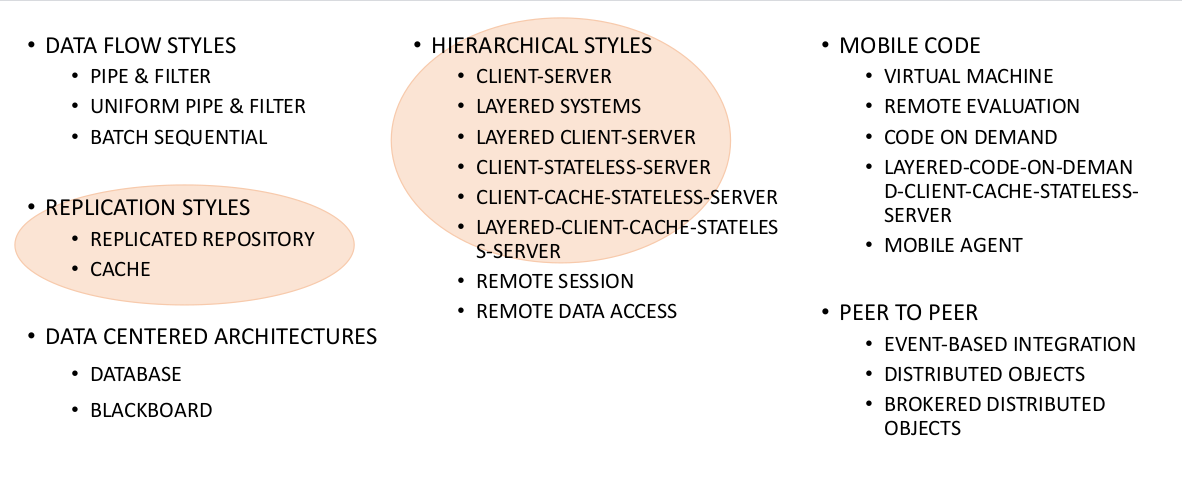
\includegraphics[width=1\textwidth]{clasificacion_arquitecturas.png}
			\caption{Clasificación de las arquitecturas}
		\end{figure}
		
		\subsection{Replication Styles}
		\subsubsection{Replicated Repository (RR)}
		Son una arquitectura en la que varios procesos brindan el mismo servicio. Los servidores descentralizados trabajan juntos para dar a los clientes la impresión de que hay un solo servidor central en lugar de un servidor centralizado.
		
		Este enfoque se emplea en sistemas de archivos distribuidos,y sistemas de control de versiones, como CVS/SVN (local), donde múltiples servidores colaboran para garantizar el rendimiento y la disponibilidad.
		
 		\paragraph{Beneficios:}
		¿Cuales son las ventajas de esto?
		\begin{itemize}	
			\item {\textbf{Escalabilidad}}: Permite manejar picos de carga, usuarios y transacciones más grandes sin comprometer el rendimiento del sistema.
			\item {\textbf{Performance}}: Como los datos se pueden obtener de los servidores más cercanos al cliente, se reduce la latencia de las solicitudes normales. Además, permite trabajar en modo offline en situaciones en las que no se puede conectar al servidor central.
			\item {\textbf{Confiabilidad}}: Una falla en uno de los servidores no causa una caída del servicio porque otros servidores pueden continuar brindando el servicio.
			
			\item {\textbf{Simplicidad}}: La simplicidad en la manipulación de datos replicados a nivel local compensa la complejidad de la replicación, lo que facilita el uso del sistema para los clientes.
		\end{itemize}
		
		Genial muy lindo, pero una preocupación importante en esta arquitectura es mantener la consistencia de los datos. Para evitar inconsistencias y conflictos, es crucial asegurarse de que los datos replicados siempre estén sincronizados y actualizados entre los servidores.
		
		\subsubsection{Cache (\$)}
		 Es una técnica de arquitectura que implica la replicación del resultado de una solicitud en un sistema, permitiendo que este resultado sea utilizado en futuras solicitudes similares. Es una variante del concepto de "Repositorios replicados" (RR) y se usa principalmente en situaciones en las que el conjunto de datos posible es mayor de lo que el cliente puede manejar o cuando el acceso completo al repositorio es innecesario.
 		\paragraph{Implementaciones}
		 
 		\begin{itemize}	
		 	\item {\textbf{Lazy Population (Población perezosa)}}: En este método, la caché se llena o actualiza solo cuando es necesario; por ejemplo, cuando un cliente hace una solicitud y el resultado no está en la caché. Esto permite ahorrar recursos al replicar solo la información necesaria.
		 	\item {\textbf{Active Population (Población activa)}}: En este caso, la caché se llena de manera proactiva, anticipando las solicitudes que es probable que se realicen en el futuro. Esta táctica tiene como objetivo mejorar aún más el rendimiento al preparar los datos antes de la solicitud.
		 \end{itemize}
		 
		 
		 \paragraph{Beneficios:}		 
			El Cache es ampliamente utilizada en aplicaciones web para mejorar el rendimiento y reducir la latencia. Algunos beneficios de su implementación son:


		 
		 \begin{itemize}	
		 	\item {\textbf{Performance}}: Aunque no ofrece mejoras tan significativas como la replicación de repositorios, aún así mejora el rendimiento del sistema al reducir el tiempo de respuesta de las solicitudes.
		 	
		 	\item {\textbf{Simplicidad}}: es más sencillo de implementar en comparación con la replicación de repositorios, lo que la convierte en una opción atractiva para sistemas con requerimientos de recursos más modestos.
		 	
		 \end{itemize}
		 
		 El cache requiere menos recursos de procesamiento y almacenamiento en comparación con la replicación de repositorios (RR), ya que solo replica datos relevantes y puede transmitir solo cuando sea necesario. Debido a la naturaleza selectiva de la caché, sin embargo, los beneficios en términos de rendimiento percibido pueden ser menores que los RR.
		 
		 
		
		
		
		\subsection{Hierarchical Styles}
		
		\subsubsection{Client Server (CS)}
		El "servidor-cliente" (servidor cliente, CS) es el estilo arquitectónico más común para aplicaciones basadas en red. El servidor y el cliente son los dos componentes principales de la arquitectura de este estilo.
		
		El componente que ofrece servicios y responde a las peticiones de los clientes es el servidor. Es responsable de enviar o rechazar las solicitudes y responder a ellas.
		
		El componente llamado cliente solicita servicios al servidor a través de un conector. El cliente sabe del servidor, pero no sabe de todos los clientes. Un servidor puede manejar a muchos clientes.
		
		 Este estilo se destaca por la clara separación de responsabilidades entre el servidor y el cliente. El cliente se encarga de solicitar servicios y el servidor de proporcionarlos. Esta separación simplifica el diseño y facilita la evolución de ambos componentes de forma independiente.
		
		\paragraph{Beneficios}
		\begin{itemize}	
			\item {\textbf{Escalabilidad}}: Debido a que el servidor es el componente que generalmente requiere una mayor capacidad y recursos para atender a múltiples clientes, la arquitectura "Client-Server" permite un crecimiento más sencillo del sistema.
			
			\item {\textbf{Simplicidad}}: La separación de funciones hace que el diseño general del sistema sea más sencillo, lo que facilita el desarrollo y mantenimiento del software.
			
			\item {\textbf{Evolucionabilidad}}: La separación de funciones permite que el cliente y el servidor evolucionen de manera independiente. Siempre y cuando se mantenga la interfaz entre ellos, las modificaciones en uno de los componentes no necesariamente afectarán al otro.
			
		\end{itemize}
		
		\subsubsection{Layered Server (LS)}
		Es un estilo arquitectónico en el que las capas jerárquicas organizan el sistema. Cada capa proporciona servicios a la capa superior mientras que la capa inferior los utiliza. Este método oculta las capas internas a las capas superiores para reducir el acoplamiento entre las diferentes partes del sistema.
 		\paragraph{Beneficios}
		\begin{itemize}	
			\item {\textbf{Evolucionabilidad}}: Permite evolucionar cada capa de manera independiente sin afectar a las demás.
			
			\item {\textbf{Extensibilidad}}: Es posible agregar nuevas capas a medida que se requieran nuevas funcionalidades o servicios en el sistema.
			
			\item {\textbf{Reusabilidad}}: Las capas pueden ser diseñadas de forma modular y reutilizarse en diferentes sistemas o contexto.
			
			\item {\textbf{Portabilidad}}: Las capas se pueden portar y utilizar en diferentes sistemas o plataformas.
		\end{itemize}
		
		Sin embargo presenta una desventaja en la \textbf{Performance}, porque la adición de capas puede introducir overhead y latencia en el sistema.
	
		
		
		
		\subsubsection{Layered Client System (LCS)}
		El enfoque arquitectónico "Cliente Servidores de capas" (LCS) combina el concepto de capas con el estilo "Cliente Servidores de capas" (CS) en sistemas basados en red. Para proporcionar una estructura más jerárquica y modular, en este caso, las arquitecturas CS se organizan en capas.
		
		El "Reverse Proxy", también conocido como proxy inverso, es una capa de aplicación accesible desde varios clientes y es un componente crucial de las arquitecturas LCS. Las solicitudes de los clientes son recibidas por esta capa y luego enviadas a los componentes del servidor. Además, el "Reverse Proxy" tiene la capacidad de traducir o modificar las solicitudes antes de enviarlas a los servidores, lo que mejora la funcionalidad.
		
		En cuestión a los beneficios, se suman los beneficios entre CS y LS.
		
		\subsubsection{Load Balancer}
		Es una parte importante de las arquitecturas de sistemas distribuidos que se encarga de recibir solicitudes (requests) de los clientes y distribuirlas entre un grupo de servidores, luego direccionando la respuesta del servidor seleccionado al cliente correspondiente. 
		
		Su objetivo principal es mejorar el rendimiento y la disponibilidad del sistema asegurándose de que el tráfico de las solicitudes se distribuya de manera equitativa y se gestione de manera eficiente entre los servidores.
		
		La relación entre el load balancer y arquitectura stateless, es que al servidor al que se envía una solicitud específica no importa, ya que cada solicitud incluye todos los datos necesarios para su procesamiento de manera independiente. Esto facilita la distribución eficiente de la carga y contribuye a la escalabilidad y la estabilidad del sistema al eliminar la necesidad de preocuparse por la persistencia del estado en los servidores individuales.
		
		
		
		
		
		
		\paragraph{Beneficios}
		\begin{itemize}	
			\item {\textbf{Escalabilidad}}: Soporta un volumen de usuarios/requests más alto.
			
			\item {\textbf{Elasticidad}}: Según el caso, podría escalar acorde a la demanda.
			
			\item {\textbf{Disponibilidad}}: Las capas pueden ser diseñadas de forma modular y reutilizarse en diferentes sistemas o contexto.
			
			\item {\textbf{Fiabilidad}}: El balanceador de carga mejora la confiabilidad del sistema al eliminar un solo punto de falla al distribuir el tráfico entre varios servidores.
			
			\item {\textbf{Performance}}: Mejor uso de los recursos escasos. En algunos casos, el balanceador de carga puede tratar ciertos tipos de solicitudes de manera diferenciada. 
			
			\item {\textbf{UX}}: Reduce el número de errores visibles por el usuario.
			
		\end{itemize}
		
		
		\subsubsection{Reverse Proxy}
		Es una parte importante de las arquitecturas de sistemas distribuidos que sirve como intermediario entre los servidores reales y los clientes. Su función principal es recibir solicitudes de clientes, reenviarlas al servidor correspondiente y devolver la respuesta del servidor al cliente. Una de sus características principales es ocultar la identidad de los servidores reales, actuando como una cara pública o fachada del sistema.
		
				
		\paragraph{Beneficios}
		\begin{itemize}	
			\item {\textbf{Seguridad}}: Actúa como una barrera de seguridad que oculta la identidad y ubicación de los servidores reales. Al hacerlo, protege los servidores de posibles ataques directos y reduce la exposición de vulnerabilidades. Esconde los servidores asi ecita explotar vulnerabilidades y puede implementar mecanismos de proteccion contra ataques DoS
			
			\item {\textbf{Escalabilidad}}: Permite una mayor flexibilidad en el manejo de recursos, ya que puede agregar o eliminar servidores reales de manera dinámica y transparente.
			
			\item {\textbf{Performance}}: Mejora el rendimiento del sistema al realizar técnicas de aceleración web, como el almacenamiento en caché, compresión y terminación SSL.	
			
		\end{itemize}
		
		\subsubsection{Client-Stateless-Server (CSS)}
		Es un método arquitectónico que proviene del estilo "Client-Server" (CS), pero tiene una limitación: no se puede almacenar el estado de la sesión en el componente servidor. En este caso, el propio cliente debe proporcionar toda la información necesaria para comprender las solicitudes del cliente, y el servidor no mantiene ningún tipo de contexto o estado de la sesión. El cliente tiene todo el control sobre el estado.
		
		¿Que es el estado? Cualquier información sobre la sesión del cliente que el servidor debe recordar y mantener entre varias solicitudes se conoce como estado.
		
		
		\paragraph{Beneficios}
		\begin{itemize}	
			\item {\textbf{Visibilidad}}: Al no mantener el estado, simplifica la tarea de un sistema de monitoreo.
			
			\item {\textbf{Confiabilidad}}: Al no depender del estado del servidor, el CSS facilita la recuperación ante fallos parciales o interrupciones.
			
			\item {\textbf{Escalabilidad}}: Permite asignar libremente un servidor para procesar una solicitud.	
			
		\end{itemize}
		
		\paragraph{Desventajas}
		\begin{itemize}
			\item {\textbf{Performance}}: Al transmitir toda la información requerida con cada solicitud, puede haber una transmisión de datos repetitiva a través de la red, lo que puede afectar el rendimiento en comparación con sistemas que almacenan el estado en el servidor.
			
		\end{itemize}
		
		\subsubsection{Client-Cache-Stateless-Server(C\$SS)}
		Es un enfoque arquitectónico que combina características de "Client Stateless Server" (CSS) y Client Cache(\$). Esta arquitectura incorpora una capa de mediadores de caché adicional para mejorar el rendimiento y la eficiencia del sistema.
		
		Los clientes interactúan con un servidor que no mantiene estado (CSS) en C\$SS, lo que significa que no almacena datos de sesión entre solicitudes. El servidor responde de manera independiente y sin dependencia de estados anteriores a cada solicitud del cliente, que contiene toda la información necesaria para ser comprendida y procesada.
		
		Sin embargo, para mejorar el rendimiento y la eficiencia, se agrega la funcionalidad de caché (Client Cache, \$) en algún lugar de la arquitectura. Los mediadores\footnote{En un sistema distribuido, los mediadores de caché, también conocidos como "proxys de caché" o "servidores de caché", son componentes que actúan como intermediarios entre los clientes y los servidores.} de caché almacenan copias temporales de respuestas a solicitudes previas para que, si un cliente hace una solicitud idéntica o similar a una que ya ha sido atendida, el servidor pueda evitar repetir todo el procesamiento y simplemente devolver la respuesta desde la caché.
		
		\paragraph{Beneficios}
		\begin{itemize}	
			\item {\textbf{Performance}}: El uso del caché para almacenar respuestas previas reduce el tiempo y los recursos necesarios para procesar solicitudes repetitivas.
			
		\end{itemize}
		
		
		\subsubsection{Layered-Client-Cache-Stateless-Server (LC\$SS)}
		Es un estilo arquitectónico que combina características de los estilos "Layered Client Server" y "Client Cache Stateless Server". Para mejorar el rendimiento, la eficiencia y la escalabilidad del sistema, se agregan componentes de proxy y caché en esta arquitectura.
		
		El LC\$SS utiliza un enfoque de capas jerárquicas donde los clientes interactúan con un servidor que no mantiene estado (Client Stateless Server, CSS), y cada solicitud del cliente contiene toda la información necesaria para comprender y procesar. Además, incluye componentes de caché que almacenan copias temporales de respuestas previamente atendidas, así como componentes de proxy que funcionan como intermediarios entre los clientes y los servidores reales.
		
		En relación a los beneficios y contras, se suman ambos aspectos de LCS y C\$SS.
		
		\subsubsection{Remote Session (RS)}
		Proviene del estilo "Client-Server" (CS) y tiene como objetivo reducir la complejidad y aumentar la reutilización de los componentes del cliente. En esta arquitectura, los clientes inician una sesión en el servidor, solicitan sus servicios y cierran la sesión al final.
		
		Es un estilo arquitectónico que simplifica la interacción del cliente con el servidor durante una sesión activa al centralizar el estado de la aplicación en el servidor.
		
				
		\paragraph{Beneficios}
		\begin{itemize}	
			\item {\textbf{Simplicidad}}: Es es más fácil de mantener y gestionar, ya que la interfaz del servidor es centralizada y los clientes solo necesitan interactuar con el servidor durante la sesión activa.
			
		\end{itemize}
		
		\paragraph{Desventajas}
		\begin{itemize}	
			\item {\textbf{Escalabilidad}}: El server requiere mantener el estado de la app.
			
			\item {\textbf{Visibilidad}}: Dado que el estado de la aplicación se mantiene completamente en el servidor, el monitor o el sistema de monitoreo debe tener acceso al estado completo del servidor.
			
		\end{itemize}
		
		
		\subsubsection{Remote Data Access (RDA)}
		Es un estilo arquitectónico que se deriva del estilo "Client-Server" (CS) y busca distribuir el estado de la aplicación entre el cliente y el servidor. En esta arquitectura, el cliente envía consultas al servidor remoto en un formato estándar, como SQL, y el servidor procesa estas consultas en un workspace para obtener un conjunto potencialmente grande de datos. Luego, el cliente puede realizar más operaciones sobre este dataset sin necesidad de transmitir todos los datos nuevamente.
		\paragraph{Beneficios}
		\begin{itemize}	
			\item {\textbf{Performance}}: Datasets grandes pueden ser reducidos del lado del
			servidor, sin transmisión de datos.
			
			\item {\textbf{Visibilidad}}: El uso de consultas de lenguaje estándar como SQL permite que el cliente y el servidor se comuniquen de manera consistente. Sin embargo, esto también podría requerir que el monitor tenga acceso al estado del servidor.
			
		\end{itemize}
		
		\paragraph{Desventajas}
		\begin{itemize}	
			\item {\textbf{Escalabilidad}}: El server requiere mantener el estado de la app.
			
			\item {\textbf{Confiabilidad}}: Si una operación falla, el workspace puede quedar en un estado desconocido.
			
		\end{itemize}
		
		
		\subsection{Mobile Code Styles}
		\subsubsection{Virtual Machine (VM)}
		Todos los estilos de Mobile Code se basan en esta arquitectura. Este método asegura la confiabilidad y la seguridad al ejecutar el código en un ambiente controlado proporcionado por la máquina virtual.
		
		Un motor de lenguaje de scripting como Perl o Python es un ejemplo común de la arquitectura de la máquina virtual. En este caso, la máquina virtual del lenguaje interpreta y ejecuta el código escrito en el lenguaje de scripting, lo que crea un ambiente controlado para la ejecución del código.
		
		\paragraph{Beneficios}
		\begin{itemize}	
			\item {\textbf{Portabilidad}}: Separa el código de su implementación/aplicación en
			una plataforma específica.
			
			\item {\textbf{Extensibilidad}}: Es más fácil crear funcionalidad sobre una plataforma
			genérica.
			
		\end{itemize}
		
		\paragraph{Desventajas}
		\begin{itemize}	
			\item {\textbf{Visibilidad}}: Es difícil saber que va a hacer un ejecutable mirando
			sólo su código fuente.			
		\end{itemize}
		\subsubsection{Remote Evaluation (REV)}
		Es una mezcla de características de "máquina virtual" (VM) y "Client-Server" (CS). En esta arquitectura, el cliente sabe cómo (know-how) ejecutar un servicio, pero carece de los recursos necesarios para hacerlo eficientemente, como CPU, memoria o acceso a una fuente de datos. El cliente envía el "conocimiento" o el código requerido al servidor para que este último lo ejecute utilizando sus propios recursos en lugar de ejecutar la operación localmente. El cliente recibe el resultado una vez que se completa la ejecución en el servidor.
		
		SQL es un ejemplo común de esta arquitectura. El cliente envía una consulta SQL al servidor en este caso, que puede leer y ejecutar el código SQL para recuperar los datos de una base de datos necesarios.
		
		\paragraph{Beneficios}
		\begin{itemize}	
			\item {\textbf{Performance}}: En lugar de usar los recursos del servidor para realizar la operación del lado del cliente, donde podría haber falta de recursos, se utilizan los recursos del servidor.
			
			\item {\textbf{Extensibilidad}}: Los componentes del servidor se pueden ajustar para satisfacer las necesidades particulares del cliente.
			
		\end{itemize}
		
		\paragraph{Desventajas}
			\begin{itemize}	
				\item {\textbf{Visibilidad}}: El cliente envía código en lugar de un simple request.			
				\item {\textbf{Escalabilidad}}: A mayor carga, mayor consumo de recursos.	
				\item {\textbf{Confiabilidad}}: El servidor tiene menos control de la ejecución.	
			\end{itemize}
		
		
		\subsubsection{Code on Demand (COD)}
		Esta arquitectura, la cual deriva de VM y CS, el cliente tiene los recursos (como CPU, memoria o acceso a una fuente de datos) para ejecutar un servicio, pero no tiene el conocimiento o la experiencia necesarios para realizar la operación de manera efectiva. El cliente envía una solicitud al servidor pidiéndole el código que representa el "know-how" necesario en lugar de enviar los datos al servidor para que se realice el procesamiento. El cliente ejecuta el código del servidor localmente para completar la operación.
		
		JavaScript (JS) en aplicaciones web es un ejemplo común de la arquitectura "Code on Demand". En este caso, el cliente tiene la capacidad de ejecutar código JavaScript, pero el servidor puede proporcionar scripts adicionales que se ejecutan localmente en el navegador del cliente para mejorar la experiencia del usuario o proporcionar funcionalidades adicionales.
		
		\paragraph{Beneficios}
			\begin{itemize}	
				\item {\textbf{Configurabilidad y Extensibilidad}}: Permite agregar nuevas funcionalidades a un cliente ya desplegado sin cambiar el código fuente original.
								
				\item {\textbf{Escalabilidad}}: Utilizar los recursos de los clientes para ejecutar el código, reduce la carga en el servidor.
				
				\item {\textbf{Performance}}: La ejecución se realiza interactuando localmente con el
				cliente, sin necesidad del servidor.
				
			\end{itemize}
		
		\paragraph{Desventajas}
			\begin{itemize}	
				\item {\textbf{Visibilidad}}: El servidor envía código al cliente en lugar de datos.			
			\end{itemize}
		
		
		
		\subsubsection{Layered Code on Demand Client Cache Stateless Server (LCODC\$SS)}
		Esta arquitectura deriva de LC\$SS + COD y se acerca más al concepto actual de la web y habla de casos en los que los navegadores permiten la ejecución de applets o extensiones de protocolos.
		
		Como ejemplo, esta arquitectura podría ser un tipo de navegador web que permite la ejecución de extensiones o applets para mejorar la funcionalidad de las páginas web.
		
		Es importante destacar no se relaciona directamente con protocolos específicos como HTTP o REST. Esto se debe a que se refiere más al concepto general de permitir que el servidor proporcione código ejecutable al cliente y que este lo ejecute localmente para aumentar sus capacidades y mejorar la interacción con el servidor o otras aplicaciones web.
		
		\subsubsection{Mobile Agent (MA)}
		Esta arquitectura combina las características REV y (COD). Un componente completo, que incluye su estado, código y datos, se mueve de un sitio remoto a otro mediante este método. Los agentes móviles pueden trabajar en ambos sentidos, es decir, pueden pasar del cliente al servidor ($c \to s$) o del servidor al cliente ($s \to  $c), dependiendo de la situación.
		
		Los agentes móviles ofrecen una gran flexibilidad en cuanto a cuándo y dónde hacer el movimiento. Por ejemplo, una aplicación en ejecución puede estar procesando una tarea específica y, en un momento determinado, decidir moverse a otra ubicación. Esto podría ocurrir para estar más cerca del próximo conjunto de datos o para aprovechar recursos específicos de otra máquina.
		
		\subsection{Peer To Peer Styles}
			\subsubsection{Event Based Integration (EBI)}
			Es un estilo de integración de componentes en el que se utiliza un enfoque Peer-to-Peer para la comunicación entre los componentes. En lugar de invocar directamente a otros componentes, un componente puede publicar uno o más eventos de esta manera. En lugar de ser invocados directamente, otros componentes se registran para recibir notificaciones sobre eventos específicos que puedan ser relevantes para vos. El sistema invoca a todos los componentes registrados cuando se produce un evento.
			
			
			Algunos ejemplos de EBI son: Smalltalk, MVC, Publisher/Subscriber.
			
			\paragraph{Beneficios}
				\begin{itemize}	
					\item {\textbf{Extensibilidad}}: Es fácil agregar nuevos componentes que respondan a
					eventos existentes o nuevos.
					
					\item {\textbf{Reusabilidad}}: Establece un mecanismo de integración y una interfaz
					de eventos común.
					
					\item {\textbf{Evolucionabilidad}}: Permite reemplazar componentes sin afectar a otros.
					
					\item {\textbf{Performance}}: En algunos sistemas, principalmente dominados por
					monitoreo, se elimina la necesidad de \textit{polling}.
					
				\end{itemize}
			
			\paragraph{Desventajas}
				\begin{itemize}	
					
					\item {\textbf{Escalabilidad}}: La cantidad de notificaciones de eventos y la tormenta de 
					eventos pueden tener un impacto en el funcionamiento del sistema. Además, si no se gestiona adecuadamente, el filtrado de eventos puede agregar complejidad y crear puntos de falla únicos en el sistema.
								
					\item {\textbf{Entendimiento}}: Difícil predecir qué ocurrirá ante un evento (ej. orden).
					Tampoco se sabe si alguien responderá.			
					
				\end{itemize}
			
			
			\subsubsection{Distributed Objects (DO)}
			Es un estilo de arquitectura Peer-to-Peer que organiza el sistema como un conjunto de componentes interactivos que actúan como pares. Este estilo representa los componentes como objetos con un estado interno oculto o protegido, así como sus operaciones asociadas. Las invocaciones de operaciones permiten que los objetos se comuniquen entre sí y pueden provocar una serie de invocaciones en otros objetos.
			
	 		Cada objeto funciona como una entidad abstracta que encapsula su estado interno y las operaciones que pueden realizar sobre ese estado. 
	 		
	 		Una operación en un objeto puede invocar operaciones en otros objetos, lo que puede dar lugar a cadenas de invocaciones que pueden extenderse a lo largo de varios objetos.
	 		
	 		El estado de la aplicación se distribuye entre los objetos del sistema, lo que permite que diferentes partes del sistema mantengan su propio estado y trabajen juntas para lograr un objetivo común.
	 		
			\paragraph{Beneficios}
				\begin{itemize}	
					\item {\textbf{Evolucionabilidad}}: Los objetos tiene interfaz pública, estado privado.
				
					
				\end{itemize}
			
			\paragraph{Desventajas}
				\begin{itemize}	
					
					\item {\textbf{Visibilidad}}: Es difícil obtener una vista general del estado y de la
					actividad del sistema.
					
				\end{itemize}
			
			\subsubsection{Brokered Distributed Objects (BDO)}
			
			Este estilo es una mezcla de los estilos "Distributed Objects" (DO) y y "Layered Client Server" (LCS). Tiene como objetivo resolver el problema de la identidad de los objetos distribuidos al agregar un intermediario (broker) que facilita la comunicación entre los objetos distribuidos.
			
			
			El problema de la identidad se reduce ya que los clientes utilizan nombres de servicio generales en lugar de identidades específicas.
			
			El broker se encarga de identificar la identidad del objeto específico al que se envía la solicitud cuando un cliente envía una solicitud con un nombre de servicio genérico.
			
			\paragraph{Beneficios}
			\begin{itemize}	
				\item {\textbf{Evolucionabilidad y Reusabilidad}}: Los nombres de servicio genéricos facilitan la reutilización y evolución de los componentes.
				
				
			\end{itemize}
			
			\paragraph{Desventajas}
			\begin{itemize}	
				
				\item {\textbf{Eficienciay Performance percibida}}: Dado que cada solicitud debe pasar a través del intermediario para que se determine la identidad del objeto específico, el uso del intermediario introduce una mayor cantidad de interacciones de red.
				
			\end{itemize}
		
		\subsection{Data Centered Architectures}
		Son un estilo arquitectónico en el que una estructura central de datos que almacena el estado del sistema es el componente principal. Este almacenamiento centralizado permite que los componentes independientes del sistema realicen sus operaciones y procesos.
		
		El  repositorio central puede variar según cómo se decida qué procesos ejecutar. El repositorio puede ser una \textbf{base de datos} que almacena los datos de entrada si el input stream decide/dispara los procesos a ejecutar.
		
		 Por otro lado, el repositorio puede ser conocido como \textbf{blackboard} si el estado actual del sistema determina qué procesos deben ejecutarse. En este caso, el repositorio es donde los componentes consultan y actualizan el estado compartido.
			\subsubsection{Blackboard}
			Es una arquitectura en la que un componente central llamado \textbf{blackboard} permite la comunicación entre múltiples fuentes de conocimiento.
				
			El blackboard funciona como una estructura de datos compartida con información sobre cómo resolver un problema. En situaciones en las que la solución de un problema complejo requiere el aporte de conocimiento de diversas fuentes, se utiliza este estilo arquitectónico.
			
			Veamos algunas características principales de esto: 
			\begin{itemize}	
				\item {\textbf{Fuentes de conocimiento}}: Son componentes independientes que tienen conocimientos específicos para abordar varios aspectos del problema. Cada fuente de conocimiento es responsable de analizar el estado actual del blackboard, proporcionar información relevante y realizar modificaciones en él.
				
				\item {\textbf{Iteraciones para llegar a la solución}}: La solución de problemas es iterativa. El blackboard se modifica mientras las fuentes de conocimiento trabajan juntas.
				
				\item {\textbf{Control coordinado por el estado del blackboard}}: La coordinación de las fuentes de conocimiento solo depende del estado actual del blackboard. Las fuentes de conocimiento responden oportunamente a los cambios del blackboard.
				
				
			\end{itemize}
				\begin{figure}[h]
					\centering
					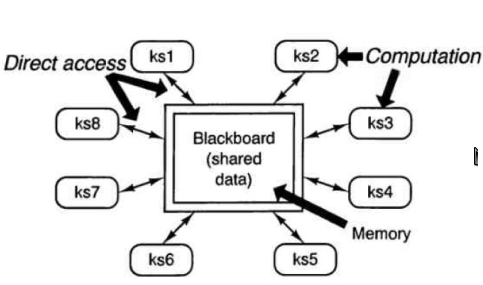
\includegraphics[width=1\textwidth]{blackboard.png}
					\caption{Representación del blackboard}
				\end{figure}
		
		\subsection{Data Flow Styles}
			\subsubsection{Pipe \& Filter (PF)}
			Este estilo se basa en la creación de flujos de datos de salida mediante el procesamiento de flujos de datos de entrada por parte de filtros independientes. El flujo de datos se procesa gradualmente y cada filtro es un componente independiente. Este estilo es adecuado para problemas que se dividen en etapas independientes y permite el desacoplamiento completo entre los filtros. Es útil para el procesamiento eficiente de grandes volúmenes de datos y facilita el desarrollo y la reutilización de componentes.
			
			Sin embargo, el flujo de datos puede estar sobrecargado y el filtro más lento puede afectar el rendimiento.
			
			Este estilo ve el sistema como una serie de transformaciones consecutivas. Es beneficioso cuando se puede abordar un problema mediante un flujo continuo de datos, como un "río". Permite medir el throughput del sistema, que es la cantidad de datos que puede procesar el sistema en un período de tiempo determinado. Una red puede ser representada por una tubería, donde la salida de un filtro puede ser la entrada de varios filtros, lo que permite un procesamiento de datos más complejo y eficiente.
			\paragraph{Beneficios}
				\begin{itemize}	
					\item {\textbf{Simplicidad}}: Se puede entender el sistema como una composición
					simple del comportamiento de los filtros individuales.
					\item {\textbf{Reusabilidad}}: Los filtros pueden reusarse y conectarse entre sí,
					siempre que estén de acuerdo con sus interfaces.
					\item {\textbf{Extensibilidad}}: Nuevos filtros pueden agregarse.
					\item {\textbf{Evolucionabilidad}}: Los filtros pueden reemplazarse por una versión
					mejorada, sin impactar en los restantes.
					\item {\textbf{Configurabilidad}}: La aplicación podría determinar los filtros a utilizar.
					\item {\textbf{Verificabilidad}}: Permiten ciertos análisis (deadlocks, throughput, etc.).
					\item {\textbf{Performance Perc.}}: Favorece el procesamiento concurrente.
				\end{itemize}
			
			\paragraph{Desventajas}
				\begin{itemize}	
					
					\item {\textbf{Performance Perc}}: Largas tuberías generan retrasos de propagación. Podría verse afectada si el problema no se adapta al flujo de datos. Si uno o varios filtros no pueden procesar sus entradas incrementalmente y deben esperar a tener todos los datos disponibles para procesarlos en batch.
					
				\end{itemize}
			
			
			
			\subsubsection{Uniform Pipe \& Filter (UPF)}
			Es una extensión del estilo "Pipe \& Filter" (PF) que incluye una restricción adicional: \textbf{todos los filtros deben tener la misma interfaz}. Con esta restricción, los filtros que se desarrollaron de manera independiente se pueden combinar libremente para crear nuevas aplicaciones.
			
			\paragraph{Beneficios}
			\begin{itemize}	
				\item {\textbf{Simplicidad}}: Más fácil entender cómo funciona un filtro (vs PF).
				\item {\textbf{Reusabilidad}}: Mayores posibilidades que en PF.
				\item {\textbf{Extensibilidad}}: Mayores posibilidades que en PF.
				\item {\textbf{Configurabilidad}}: Mayores posibilidades que en PF.
				\item {\textbf{Visibilidad}}: Es más fácil para un componente monitorear la
				interacción entre dos filtros cualesquiera.
			\end{itemize}
			
			\paragraph{Desventajas}
			\begin{itemize}	
				
				\item {\textbf{Performance}}: Los datos podrían requerir ser convertidos desde/hacia el
				formato original/definido por la interfaz.
				
			\end{itemize}
			
			\subsubsection{Batch Sequential}
			
			Es similar a "Pipe \& Filter" (PF) o "Uniform Pipe \& Filter"(UPF) pero con una diferencia clave: cada filtro debe terminar su procesamiento antes de que comience el siguiente filtro. Esto hace más sencillo dividir el sistema en subsistemas independientes, pero puede aumentar la latencia y reducir el throughput. Además, disminuye las oportunidades de competición en el procesamiento de datos. 
			
		
		
		\subsection{La Web}
		Es probable que, cuando nos pregunten que es la web, pensemos en el internet, pero ¿son lo mismo?
		\subsubsection{¿La Web = Internet?}
		La respuesta es no, no son lo mismo. 
		El internet es un sistema de redes de computadoras interconectadas. Mientras que la Web es un sistema de documentos \textbf{hipertexto} interrelacionados, accedidos a traves de internet. Podríamos ver a la web como una aplicacion "corriendo" sobre internet.
		
		\subsubsection{Atributos de calidad}
		\begin{itemize}		
			\item \textbf{Low Entry-barrier (Usability)}: Cualquier persona puede contribuir y participar en la Web porque la creación de información es voluntaria.
			
			\item \textbf{Extensibilidad}: La web debe ser capaz de adaptarse y incorporar nuevas funcionalidades a medida que se desarrolla.
			
			\item \textbf{Disponibilidad}: La web puede presentar condiciones adversas y las mejores aplicaciones construidas sobre la web deben poder resistir a ellas.
			
			\item \textbf{Internet-Scale}
			\begin{enumerate}
				\item \textbf{Anarchic Scalability}: La web debe ser capaz de adaptarse y incorporar nuevas funcionalidades a medida que se desarrolla. Las relaciones a largo plazo y la coordinación centralizada entre los componentes del sistema no existen en la Web. Los clientes no pueden conocer todos los servidores y los servidores no pueden mantener un estado entre solicitudes.	
				
				\item \textbf{Independent Deployment:}: Las partes del sistema de la Web pueden evolucionar a diferentes ritmos.
			\end{enumerate}
			
			\item \textbf{Distributed Hypermedia (Hipertexto Distribuido)}: Las instrucciones sobre qué se puede hacer con los datos se trata igual que a los datos. Tanto los datos como sus instrucciones son manejadas por el server.

			
		\end{itemize}
		
		\subsection{REST}
		Es un estilo arquitectónico para diseñar sistemas de software que se utilizan ampliamente en aplicaciones web y servicios web.
		
		Los sistemas se consideran colecciones de recursos que se pueden identificar a través de URLs en el contexto de REST. Cada recurso es una entidad o un conjunto de datos que se puede acceder, crear, actualizar o eliminar a través de las operaciones estándar de HTTP, como GET (obtener), POST (crear), PUT (actualizar) y DELETE (eliminar). Estas operaciones se realizan mediante solicitudes HTTP a través de la web.
		\begin{figure}[h]
			\centering
			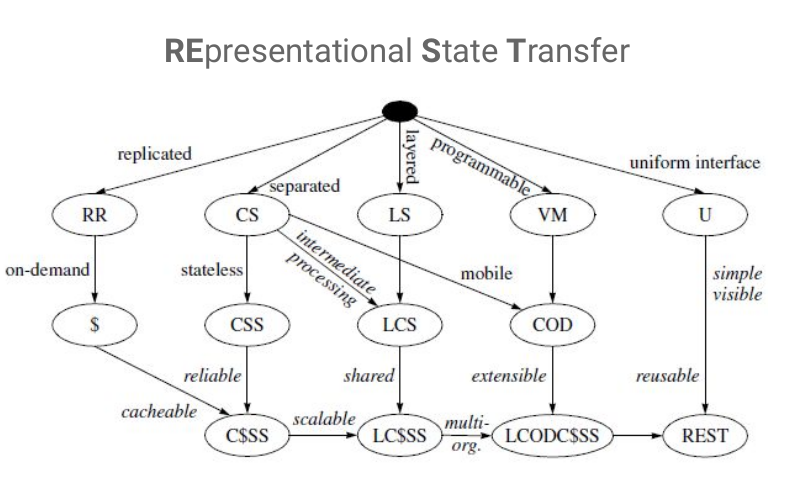
\includegraphics[width=1\textwidth]{arquitectura_rest.png}
			\caption{Arquitectura REST}
		\end{figure}
		
		La característica principal de REST es la interfaz uniforme (Uniform Interface), que establece un conjunto de reglas que todos los servicios web basados en REST deben seguir. Las siguientes tácticas son:
		\subsubsection{Uniform Interface}
		\begin{itemize}		
			\item \textbf{Identificación de Recursos}: Todo recurso debe tener 1 ID y el ID puede cambiar. (Simplicity, Visibility, Reusability).
			
			\item \textbf{Los métodos de acceso con misma semántica}: todas las operaciones de acceso (métodos) tienen el mismo significado y comportamiento para todos los recursos en el sistema. (Visibility, Scalability y Availability (posibilita LS y \$)).
			
			\item \textbf{Manipulación de Recursos a través de Representaciones}: Los recursos pueden tener múltiples representaciones, como JSON, XML o HTML. Capturan el estado actual ó deseado de un recurso. Se transfieren entre componentes. (Simplicity, Visibility, Reusability,
			Evolvability (information hiding)).
			
			\item \textbf{Mensajes Auto-descriptivos}: Cada mensaje HTTP debe ser autodescriptivo y contener toda la información que el servidor necesita para comprender y procesar la solicitud. (Visibility, Scalability y Availability (posibilita LS y \$), Evolvability (extensible communication))
			
			\item \textbf{HATEOAS (Hipertexto como Motor de Estado de la Aplicación)}: En las respuestas, el servidor debe proporcionar enlaces a otros recursos relacionados. Esto permite que el cliente explore y navegue a través de los enlaces hipertexto de la aplicación. (Simplicity, Visibility, Reusability, Evolvability (loose coupling), Adaptable (late binding of application transitions))
		\end{itemize}
		
		
		\subsubsection{Application State y Resource State}
		La información sobre "dónde está" o en qué punto se encuentra un cliente durante su interacción con el servidor se refiere al Application State en REST. En otras palabras, el Application State indica el estado actual de la aplicación del cliente mientras interactúa con el servidor. (Esta del lado del cliente)
		
		Por otro lado, el Resource State se refiere al estado de un recurso específico que está almacenado en el servidor y que puede ser modificado a través del envío de representaciones o datos al servidor mediante solicitudes HTTP.

		¿Y esto como se relaciona bien con REST? 
		
		Bueno, en REST,  Application State y el Resource State se manejan de manera independiente. El servidor no almacena datos sobre el estado de la aplicación para cada cliente porque REST es una arquitectura sin estado. Por el contrario, el estado de la solicitud se almacena en el cliente y se envía al servidor para cada solicitud relevante. El servidor responde con el estado de recursos actualizado en respuesta a la solicitud del cliente.
		
		\subsubsection{HyperMedia}
		
		En REST este concepto es clave, Hypermedia significa que la información de control de aplicación puede estar dentro o sobre la presentación de la información. Esta información sobre el control de aplicación se representa en un lenguaje que las máquinas pueden leer y se utiliza para conectar recursos y describir sus capacidades.
		
		Permite la navegación y la interacción entre recursos mediante enlaces (links). Los enlaces son relaciones hypermedia que permiten organizar la información de manera adaptable y brindan instrucciones sobre cómo usar la información en la aplicación. Estos enlaces permiten que el servidor muestre al cliente un menú de opciones que le permite acceder a recursos relacionados o realizar acciones específicas.
		
		La presencia de Hypermedia en las respuestas del servidor permite que el cliente interactúe dinámicamente con la aplicación, lo cual permite que el cliente decide qué es lo que va a pasar.
		
		
		
		\section{SDGT y SOA}
		
		\subsection{SDGT}
			Los sistemas de software distribuidos de gran tamaño (SDGT) son complejos, heterogéneos y de gran escala. Estos sistemas se pueden encontrar en una variedad de empresas y organizaciones, desde aplicaciones comerciales hasta infraestructuras de telecomunicaciones.
			
			Algunas de las características de SDGT son: 
			\begin{itemize}		
				\item \textbf{Legacy}: Muchos de estos sistemas han cambiado con el tiempo y pueden incluir tecnologías y componentes más antiguos que todavía son necesarios para su funcionamiento.
				
				\item \textbf{Heterogéneos}: Los SDGT suelen estar compuestos por múltiples tecnologías, plataformas y sistemas que deben colaborar para realizar sus funciones.
				
				\item \textbf{Larga Vida}: Estos sistemas deben mantenerse y adaptarse a lo largo del tiempo para mantenerse útiles durante mucho tiempo.
				
				
				\item \textbf{Complejos}: Los SDGT son complejos porque deben integrar numerosos componentes, servicios y datos para brindar una funcionalidad completa.
				
				\item \textbf{Diferentes Owners}: En estos sistemas distribuidos, diferentes equipos o departamentos pueden ser responsables de diferentes partes del sistema.
				
				\item \textbf{Información Redundante}: Debido a su evolución y crecimiento a lo largo del tiempo, los SDGT pueden contener información redundante o duplicada.
				
				\item \textbf{Necesidad de Escalar}: La demanda de estos sistemas puede aumentar con el tiempo, lo que significa que es necesario aumentar su capacidad para mantener un rendimiento adecuado.
				
			\end{itemize}
		
		La tecnología de la información (IT) es esencial para el éxito de las organizaciones en el entorno empresarial actual. La adaptabilidad y la flexibilidad son esenciales para lidiar con los cambios y los desafíos que enfrentan los negocios. Para abordar la creciente complejidad y mantener el ritmo de la innovación, los SDGT se vuelven necesarios.
		
		Pero, los SDGT también enfrentan dificultades significativas. Un factor a tener en cuenta es la deuda técnica, que hace referencia a los problemas acumulados por la toma de decisiones técnicas subóptimas. Además, debido a la complejidad y la interdependencia de sus componentes, el mantenimiento de estos sistemas puede ser costoso y riesgoso.
		
		\subsection{SOA}
		\textit{"La arquitectura orientada a servicios (SOA) es un paradigma para la realización y el mantenimiento de procesos empresariales que abarcan grandes distribuidos".}
		
		Es un método arquitectónico para la creación de sistemas de software que se centra en la creación y ejecución de servicios. 
		
		
		\subsubsection{Servicios}
		Estos servicios son unidades de funcionalidad autocontenidas que representan una acción o un conjunto de acciones relacionadas con la empresa. Cada servicio tiene una interfaz clara que explica sus funciones y cómo se puede acceder a ellas.
		
		\paragraph{¿Cuales son los aspectos claves?}
		\begin{itemize}		
			\item \textbf{Funcionalidad de negocio auto-contenida}: Cada servicio representa una función única que agrega valor al negocio. Estos servicios pueden ser básicos, como actualizar una dirección, o complejos, como procesar un pedido completo.
			
			
			\item \textbf{Interfaz bien definida}: Cada servicio tiene una interfaz clara que permite a los clientes interactuar con él. Detalles como los métodos o funciones disponibles, los formatos de datos aceptados y las restricciones de uso (SLA) se encuentran en esta interfaz.
			
			
			\item \textbf{Solución del gap entre IT/business}: La SOA tiene como objetivo ayudar a las empresas a alinear la tecnología de la información (IT) con las necesidades comerciales.
			
			
			\item \textbf{Composición de servicios}: Los flujos de trabajo complejos se pueden crear utilizando los servicios de SOA individualmente o en conjunto. La composición de servicios permite la reutilización de servicios existentes para crear aplicaciones más grandes y complejas.
			
		\end{itemize}
		
		\paragraph{Atributos}
			\begin{itemize}		
				\item \textbf{Autocontenido}: Los servicios de SOA deben ser autónomos, autónomos e independientes. Esto significa que cada servicio debe ser lo más independiente posible de otros y no depender de otros para que funcione. Están hechos para que varios propietarios o clientes los usen.
								
				\item \textbf{Coarse-Grained}: En lugar de realizar tareas individuales muy pequeñas, los servicios en SOA suelen ser de grano grueso. Esto permite una mayor abstracción y flexibilidad, pero también puede afectar el rendimiento.
					
				\item \textbf{Visible}: Para llamar a un servicio, debes saber si existe y tener acceso a su interfaz				
				
				\item \textbf{Stateless}: Los servicios en SOA se prefieren idealmente que no mantengan estado entre las solicitudes. Sin embargo, esto puede ser difícil de lograr en algunas circunstancias y se pueden tener servicios estatales.
				
				\item \textbf{Idempotente}: Los servicios deben ser idempotentes, lo que significa que ante la duda, permitir enviar la misma solicitud reiteradas veces
				
				\item \textbf{Reusable/Componible}:  el objetivo es evitar la redundancia y fomentar la reutilización de los servicios. Los procesos comerciales deben dividirse en partes más pequeñas y reutilizables que se pueden agregar para crear funcionalidades más complejas.
				
				\item \textbf{Technical Services}: Existen servicios técnicos que son necesarios para el funcionamiento del sistema aunque no están relacionados con el negocio en sí.
								
				\item \textbf{Interoperable}: Los servicios deben ser interoperables, lo que significa que pueden ser llamados desde otros sistemas y plataformas.
				
			\end{itemize}
		
		\subsubsection{Enterprise Service Bus (ESB)}
		Un Enterprise Service Bus (ESB) es la infraestructura de SOA; su objetivo es proporcionar interoperabilidad (conectividad datos y enrutamiento) combinada con  algunos servicios adicionales como seguridad supervisión, etc.
		
		\paragraph{Conexiones}
		\begin{itemize}		
			\item \textbf{Conexión punto a punto}: Permite que el consumidor se conecte directamente con el proveedor del servicio al conocer su dirección (endpoint).
			\begin{figure}[h]
				\centering
				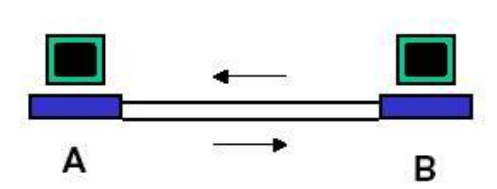
\includegraphics[width=0.5\textwidth]{punto_punto.png}
				\caption{Conexión punto a punto}
			\end{figure}
			
			
			\item \textbf{Conexión indirecta (Mediador)}: El consumidor solicita un servicio mediante tags en lugar de conocer directamente la dirección del proveedor. El bus de servicios empresariales (ESB) sirve como intermediario y envía la solicitud al servidor adecuado. Esto hace que la infraestructura sea menos acoplada y permite cambios dinámicos. 
			
			\item \textbf{P2P + Name Server}: Cuando se utiliza la conexión punto a punto, esta es una alternativa. La implementación de la indirección se lleva a cabo mediante el uso de un name server, que almacena las direcciones físicas de cada servicio.
							
			
			\item \textbf{P2P + Interceptor/Proxy}: El proveedor de servicio es sustituido por un Load Balancer o interceptor que recibe los mensajes del consumidor. Ante la recepción de un mensaje, deriva el pedido a un proveedor de servicio que conoce, lo que permite la implementación de la tolerancia a fallos y el balanceo de carga. Además, los interceptores pueden brindar servicios adicionales, como protección y vigilancia.
		
			
		\end{itemize}
		
		\paragraph{Clasificación:} SOA con ESB se puede clasificar en dos categorías principales
		\begin{itemize}		

			\item \textbf{Protocol-Driven}: El ESB establece un protocolo de comunicación para conectar a los clientes con los proveedores de servicios. Ej. Web Services \& SOAP.
			
			\item \textbf{API-Driven}: El ESB establece las interfaces de programación de aplicaciones (API) de la plataforma que interactúan con los servicios. Ej. interfaces Java.
			
		\end{itemize}
		
			
		\paragraph{Valores agregados} SOA con ESB se puede clasificar en dos categorías principales
		\begin{itemize}		
			
			\item \textbf{Data Mapping}: Puede facilitar la transformación de datos entre formatos definidos por varios servicios.
			
			\item \textbf{Ruteo Inteligente}: Puede administrar la tolerancia a fallos, optimizar el balanceo de carga entre los diferentes servicios y realizar un ruteo inteligente de mensajes. Además, puede priorizar los mensajes según los estándares de su empresa.
			
						
			\item \textbf{Seguridad}: Puede proporcionar mecanismos de seguridad para limitar el acceso a ciertos servicios, permitiendo que solo los clientes autorizados los usen.
			
			
			\item \textbf{Reliability (Fiabilidad)}: Puede aumentar la confiabilidad de ciertos protocolos de comunicación mediante la implementación de mecanismos de gestión de errores y garantizar la recepción de mensajes.
			
						
			\item \textbf{Monitoring \& Logging}: Permite realizar el seguimiento y registro de la actividad del sistema distribuido.
			
			\item \textbf{Actividad del Negocio}: Puede analizar el estado del negocio en tiempo real, detectando comportamientos inusuales y creando oportunidades comerciales.
			
			
		\end{itemize}
		
		
		
		
		\section{Cloud Computing Architecture}
		Es un modelo para permitir el acceso ubicuo, conveniente, y bajo demanda a un conjunto compartido de recursos computacionales configurables (redes, servers, almacenamiento, aplicaciones, y servicios) a través de la red, que pueden ser rápidamente provistos y desplegados con un esfuerzo mínimo de administración o de interacción con el proveedor del servicio.
		
		\subsection{Características}
		
		\begin{itemize}
		
			\item {\textbf{On-Demand usage}}: Permite a los clientes acceder a los recursos de manera unilateral sin que los proveedores intervengan manualmente. Los usuarios pueden abastecerse automáticamente de recursos según sus necesidades.
		
			\item {\textbf{Ubiquitous Access}}: Varios protocolos e interfaces de acceso permiten que los recursos en la nube sean accesibles desde una amplia gama de dispositivos. El acceso a los recursos debe tener en cuenta la seguridad.
		
			\item {\textbf{Multitenancy}}: Un solo software o servicio en la nube puede atender a muchos clientes al mismo tiempo y mantener a cada consumidor aislado. Esto se logra mediante la compartición de recursos.
		
			\item {\textbf{Elasticity}}: Según las necesidades de carga, la nube permite la escala automática y dinámica de los recursos. Para escalar los recursos hacia arriba o hacia abajo, se pueden establecer condiciones predeterminadas o basadas en eventos en tiempo real.
			
			\item {\textbf{Measured Usage}}: El uso de los recursos informáticos se monitorea y registra minuciosamente. El modelo "Pay-as-you-go", también conocido como "pago por uso", permite que los usuarios paguen solo por los recursos que han utilizado. El monitoreo continuo de los recursos también ayuda a generar reportes y análisis.
			
			
			\item {\textbf{Resiliency}}: La distribución redundante de los recursos en la nube aumenta la disponibilidad y la resiliencia ante fallas o desastres.
			
		\end{itemize}
		\subsection{Planificación de la capacidad}
		En la gestión de sistemas y recursos informáticos, la planificación de la capacidad es un proceso esencial para garantizar un rendimiento óptimo y satisfacer las demandas de los usuarios. Para elegir cuándo agregar capacidad, hay tres métodos principales.
		\begin{enumerate}
			
			\item {\textbf{Lead strategy}}: Antes de que ocurra un aumento significativo en la carga del sistema, se anticipa la demanda futura y se agrega capacidad. El objetivo es prever el crecimiento y asegurarse de que los recursos estén disponibles para manejarlo de manera efectiva.
			
			\item {\textbf{Lag strategy}}: La capacidad se agrega cuando los recursos se utilizan al máximo o incluso cuando la sobrecarga del sistema daña el rendimiento del sistema.
			
			\item {\textbf{Match strategy}}: Los incrementos y decrementos de capacidad se realizan en cantidades limitadas y se ajustan según la demanda real.
			
		\end{enumerate}
		
		\subsection{Delivery Models}
		Los modelos de entrega son diversas formas en que los proveedores de servicios cloud proporcionan y entregan recursos y servicios a los usuarios. Estos modelos ofrecen una combinación única y pre-empaquetada de recursos y funciones.
		
		Hay 3 tipos de delivery models:
		\begin{enumerate}
			
			\item {\textbf{IaaS}}: El hardware, las redes, el almacenamiento y los sistemas operativos se proporcionan por el proveedor de cloud computing. Los usuarios tienen un gran control sobre estos recursos y pueden acceder a ellos a través de Internet. Ej: AWS, Azure, OpenStack.
			
			\item {\textbf{PaaS}}: La plataforma completa del proveedor de nube incluye infraestructura, sistemas operativos, entorno de desarrollo, herramientas y servicios para el desarrollo, prueba y despliegue de aplicaciones. Ej: Azure (.NET), Google App Engine.
			
			\item {\textbf{SaaS}}: El software proporcionado por el proveedor de cloud se distribuye a los usuarios a través de Internet. Sin necesidad de instalar o mantener el software localmente, los usuarios pueden acceder a estas aplicaciones y utilizarlas a través de un navegador web. Ej: Google Apps, Salesforce.
			
		\end{enumerate}
		
		\subsection{Deployment Models}
		Se refieren a los diversos tipos de ambientes de cloud según quién los posee, su tamaño y cómo los usuarios los pueden acceder. Estos modelos pueden variar según las necesidades y requisitos específicos de cada organización, pero establecen cómo se implementa y gestiona la infraestructura y los servicios cloud.
		
		
		Los siguientes son los modelos de implementación principales para la computación cloud:

		\begin{enumerate}
			
			\item {\textbf{Public Cloud}}: Un proveedor de cloud proporciona infraestructura y servicios de cloud que están disponibles para el uso público a través de Internet.

			\item {\textbf{Private Cloud}}: Los servicios cloud y la infraestructura son propiedad exclusiva de una sola organización. Puede estar alojado en la sede de la organización o en un centro de datos dedicado.
			
			
			\item {\textbf{Community Cloud}}: Un proveedor de cloud proporciona infraestructura y servicios de cloud que están disponibles para el uso público a través de Internet.
			

				
			\item {\textbf{Hybrid Cloud}}: s una mezcla de nubes privadas y públicas que están conectadas y funcionan como una infraestructura única.
			
		\end{enumerate}
		
		\subsection{Estilos de arquitecturas habituales}
		
		\subsubsection{N-tier}
		Es un enfoque común en el diseño de sistemas de software y aplicaciones que divide las funcionalidades del sistema en capas físicamente separadas y bien definidas. Cada capa realiza un conjunto de tareas específicas y se comunica con las capas cercanas a través de interfaces bien definidas. 
		
		Cada capa puede escalar horizontalmente agregando más instancias o recursos para manejar una mayor carga de trabajo
		
		
		\subsubsection{Web-Queue-Worker}
		Es una variante del patrón de arquitectura de capas N-tier y es comúnmente utilizado para implementar sistemas que manejan tareas en serie, tareas de larga duración y tareas de uso intensivo de recursos. Este patrón se basa en tres partes principales: la interfaz de usuario (front-end), la cola (queue) y los trabajadores.
		
		\textbf{El front-end} es la capa de presentación y UI del sistema. Puede ser una aplicación web, móvil o otra forma de interacción con el usuario. El front-end de este patrón no almacena información sobre el estado del usuario o la sesión.
		
		\textbf{La cola} es un método para encolar y desencolar las tareas. En lugar de procesar la solicitud de inmediato, el front-end la encola en la cola para su posterior procesamiento. 
		
		\textbf{Los workers} son los procesos o servicios que consumen tareas en segundo plano y las procesan en la cola. Los workers son stateless y están construidos para ser extremadamente escalables y tolerantes a fallas. Para manejar una mayor carga de trabajo, pueden ejecutarse en múltiples instancias o servidores. Cada worker toma una tarea de la cola, la procesa y luego la marca como completa.
		
		Este tipo de arquitectura es particularmente útil para sistemas que deben manejar tareas complejas o una gran cantidad de trabajo porque permite escalar horizontalmente tanto el front-end como los empleados para satisfacer la creciente demanda de tareas.
		
		
		\subsubsection{Event-driven}
		Es una forma de diseñar sistemas distribuidos en los que los eventos comunican las partes del sistema. En este patrón, los consumidores (o subscriptores) reaccionan a los eventos para realizar acciones específicas, y los productores generan eventos que representan cambios o sucesos importantes en el sistema.
		
		Los productores y los consumidores no necesitan conocerse directamente porque están desacoplados entre sí. Los productores y los consumidores no son conscientes de qué componentes están produciendo los eventos.
		
		Los clientes de eventos también están desconectados. Cada cliente ve todos los eventos que se producen, pero decide por sí mismo cómo responder a cada uno.
		
		\paragraph{Modelos}
		\begin{itemize}
			\item {\textbf{Pub/sub}}: Los eventos se envían an un canal central, que puede ser un bus de eventos o un tema, y los clientes pueden suscribirse an este canal para recibir los eventos que les interesen. Los nuevos subscriptores no pueden ver los eventos anteriores, por lo que no se pueden reproducir. 
			\item {\textbf{Event Streaming}}: Los eventos se escriben en un registro persistente y ordenado. Los clientes pueden leer los eventos de cualquier parte del flujo, lo que les permite reproducir eventos anteriores si es necesario.
		\end{itemize}
		
		
		\subsubsection{Micorservices}
		Son un enfoque arquitectónico en el que una aplicación monolítica se divide en servicios más pequeños, autónomos y desacoplados, cada uno encargado de una función o área funcional específica de la empresa. Cada microservicio funciona en su propio entorno y tiene su propio código fuente, lo que permite su despliegue independiente y manejo por un pequeño grupo de desarrolladores.
		
		Los microservicios no tienen dependencias directas entre sí, pero se comunican entre sí a través de APIs. Esto permite que cada microservicio se desarrolle y se actualice sin interferir con los demás.
		
		Ofrecen tolerancia a fallos, lo que significa que si un microservicio falla, no afectará el funcionamiento de toda la aplicación porque están diseñados para ser resistentes y recuperarse de manera independiente. Además, los microservicios pueden escalarse de manera independiente según las necesidades de carga de trabajo, y un servicio de balanceo de carga puede redirigir solicitudes a los microservicios adecuados para lograr una distribución equilibrada de la carga. Esto permite la escalabilidad y el balanceo de carga flexibles. 
		
		Además, los microservicios no están limitados an una sola tecnología, lo que significa que cada microservicio puede utilizar la tecnología más adecuada para su función particular. Un mecanismo de descubrimiento de servicios, que asigna servicios a los nodos y permite identificar fallas y reequilibrar los servicios según sea necesario, es necesario para que los microservicios se comuniquen entre sí.
		
		\subsection{Usage Patterns}
		\subsubsection{Auto-Scaling}
		Consiste en implementar un proceso de asignación dinámica de recursos, como nodos, almacenamiento y colas, para adecuar la capacidad de la aplicación a la demanda en tiempo real, siguiendo una estrategia de "match strategy".
		
		Esto favorece a la Performance, Scalability, Elasticity.
		
		\paragraph{Consideraciones para la implementación:} 		
		El sistema debe ser stateless y escalable horizontalmente para evitar la dependencia de instancias específicas.
		
		\paragraph{Buenas practicas} 		
			\begin{enumerate}
				\item Usar las características de escaneo automático proporcionadas por el proveedor de la nube, ya que crear una solución personalizada requeriría mucho trabajo. 
				\item Escalar cada componente o subsistema por sí solo para aumentar la flexibilidad y la eficiencia.
				\item establecer límites inferiores y superiores en las reglas de autoescala para evitar escalamientos excesivos o innecesarios.
				\item Tener en cuenta las tareas de larga duración que podrían afectar el escalamiento y, si es posible, refactorice hacia un patrón de tuberías y filtros o utilice puntos de control en un almacenamiento externo para administrar tareas en progreso.
			\end{enumerate}
		
		\subsubsection{Queue-Based Load Leveling}
		Este patrón se puede implementar para evitar la sobrecarga de un servicio que está sujeto a cargas grandes e intermitentes. Este método implica la creación de una cola de mensajes entre los clientes del servicio y el propio servicio, generalmente una cola FIFO. La cola funciona como un buffer, almacenando temporalmente los mensajes antes de que el servicio los procese.
		Algunos beneficios de este patrón son los siguientes:
			\begin{enumerate}
				\item Incluso en situaciones de alta demanda, asegura que cada mensaje se envíe al menos una vez. 
				\item Permite ajustar la cantidad de colas y servicios según la demanda, lo que aumenta la flexibilidad y la capacidad de escala.
				\item establecer límites inferiores y superiores en las reglas de autoescala para evitar escalamientos excesivos o innecesarios.
				\item La comunicación es unidireccional, lo que significa que el servicio procesa los mensajes de los clientes en orden de llegada.
			\end{enumerate}

		Sin embargo, es importante tener en cuenta que este patrón por sí solo no es suficiente si se espera que el servicio responda a los mensajes enviados.
		
		Esto favorece a la Availability, Performance, Scalability.
		
		\subsubsection{Competing Consumers}
		Este patrón se puede utilizar para lograr que múltiples componentes "consumers" (workers) procesen mensajes de múltiples  "producers" (apps) de forma concurrente. Este método establece una cola de mensajes entre las instancias de los productores y las instancias de los consumidores. Cada app instance puede enviar mensajes a la cola, y cualquier worker en un pool de workers puede procesar estos mensajes de manera competitiva.
		
		Algunos beneficios de este patrón son los siguientes:
		\begin{enumerate}
			\item \textbf{Procesamiento asíncrónico}: los mensajes se procesan de forma asíncrona, lo que permite a los empleados trabajar juntos sin esperar respuestas inmediatas.
			
			\item \textbf{Garantiza de entrega}: La cola garantiza que cada mensaje sea entregado al menos una vez, lo que garantiza "al menos una vez de procesamiento".
			\item \textbf{Escalabilidad y disponibilidad}: Los trabajadores pueden escalar horizontalmente para manejar una gran cantidad de solicitudes, y gracias a la redundancia, el sistema sigue funcionando correctamente si un trabajador falla.
			\item \textbf{Alta disponibilidad}: si un trabajador falla durante el procesamiento de un mensaje, este vuelve a la cola y puede ser tomado por otro trabajador.
			\item \textbf{Sin coordinación}: No es necesaria la coordinación entre los empleados ni entre las aplicaciones y los empleados, lo que simplifica la arquitectura y aumenta la flexibilidad.		
				
		\end{enumerate}
		
		
		Esto favorece a la Availability, Performance, Scalability.
		
		\subsubsection{Priority Queue}
		Se puede utilizar una cola de prioridad o cola de prioridad para priorizar solicitudes y respetar diferentes SLAs para clientes particulares. En esta cola, en lugar de seguir el orden de llegada normal (FIFO - First-In-First-Out), los mensajes se ordenan según su nivel de prioridad. De esta manera, los pedidos con alta prioridad se procesarán antes que los de baja prioridad, sin importar el orden en que lleguen.
		
		Un cliente recibe prioridad según sus necesidades y SLAs específicos. Los mensajes se insertan en la cola de acuerdo con esta prioridad, y los empleados o clientes procesan los mensajes de acuerdo con su nivel de prioridad. Esto garantiza que las solicitudes de alta prioridad sean atendidas rápidamente, incluso si llegan después de solicitudes de baja prioridad.
		
		Esto favorece a la Performance, Scalability.
		
		\subsubsection{Health Endpoint Monitoring}
		Este patrón sirve para verificar si un servicio esta cumpliendo con el nivel requedo de availability y performance. Implica la implementación de un punto de control de salud, también conocido como healt endpoint, en el servicio. Este punto de control proporciona información sobre el estado del servicio y responde a solicitudes específicas.
		
		Si es necesario para garantizar la seguridad del servicio, el monitoreo de los healt endpoints se puede realizar desde una variedad de ubicaciones. Además, es posible incorporar pruebas automáticas en el healt endpoint para que el propio servicio realice pruebas automáticas para verificar su salud y funcionalidad.
		
		
		Esto favorece a la Performance, Availability.
		
		\subsubsection{Retry}
		Este patrón sirve para manejar fallas temporales de los servicios que consumen. Implica la implementación lógica de reintentos (retry) que consideren un lapso de tiempo(delay) entre cada reintento. Este punto de control proporciona información sobre el estado del servicio y responde a solicitudes específicas.
		
		La definición de una política de reintentos adecuada debe tener en cuenta la cantidad de reintentos y el tiempo que transcurre entre ellos. La política de repetición debe ajustarse al tipo de interacción cliente-servidor para evitar una sobrecarga del servicio. Los reintentos son menos peligrosos si la operación es idempotente (no tiene efectos secundarios cuando se repite).
		
		Mantener registros de intentos fallidos ayuda a detectar y analizar problemas futuros. Una política de reintentos bien planificada puede mejorar la experiencia del usuario al manejar de manera más elegante las fallas temporales que pueden ocurrir en entornos cloud u otros entornos distribuidos.
		
		
		Esto favorece a la Availability.
		
		\subsubsection{Circuit Breaker}
		Este patrón sirve para evitar que las aplicaciones invoquen servicios que están caídos y detectar cuando el problema está resuelto. Implica la implementación de un proxy que registre la	cantidad de fallas recientes y use esos	datos para decidir si invocar el servicio o	si fallar inmediatamente.
		
		El Circuit Breaker tiene tres estados principales:
			\begin{enumerate}
				\item \textbf{Closed}: Pasan todos los requests.
				
				\item \textbf{Open}: Devuelve excepción inmediatamente.
				\item \textbf{Half-Open}: Un número limitado de	requests pasan, los otros fallan.
			
			\end{enumerate}
		
		Esto favorece a la Availability.
		
		\subsubsection{Throttling}
		Este patrón sirve para controlar el uso de recursos para cumplir con SLAs sin utilizar unicamente auto-scaling. Implica en imponer un limite al uso de recursos, que al alcanzarse, el sistema comenzará a regular los requests de los clientes.
		
		Para implementar el throttling, se pueden rechazar las solicitudes de clientes que han excedido el límite establecido durante un cierto período de tiempo, degradar o deshabilitar funcionalidades no esenciales para liberar recursos o priorizar las solicitudes según los acuerdos de nivel de servicio (SLA) para dar prioridad a las solicitudes de alta prioridad.
		
		Esto favorece a la Availability, Performance.
		
				
		\subsubsection{Sharding}
		Este patrón sirve para superar las limitaciones de espacio, recursos, ancho de banda y geograficas de un almacenamiento de datos en 1 server. Implica en dividir el almacenamiento de datos en particiones "horizontales" (shards).
		
		Cada shard funciona en su propio servidor y es independiente del resto, lo que permite escalar horizontalmente y equilibrar la carga entre shards. La ubicación geográfica de los shards también puede optimizarse para estar cerca de los usuarios que accederán a los datos.
		
		Cada shard contiene un conjunto de datos que pertenecen a un rango determinado por una clave de shard o clave de partición. Existe una variedad de enfoques para asignar los datos a los shards, incluida la estrategia de mapa de shardkey-shard, la estrategia de rango que agrupa elementos relacionados o la estrategia de hash que usa una función de hash para asignar los datos.
		
		Esto favorece a la Availability, Performance.
		
		
		\section{Base de datos relacionales}
		Una base de datos relacional es un tipo de sistema de gestión de bases de datos (DBMS) que organiza y almacena datos en forma de tablas conectadas. Es una solución para la gestión y recuperación de datos estructurados.
		
		
		\subsection{Beneficios}
		\begin{itemize}
			\item {\textbf{Almacenamiento}}: Capacidad para manejar grandes volúmenes de información y flexibilidad para almacenar y buscar fragmentos de datos de manera eficiente.
			
			\item {\textbf{Modelo (casi) estándar}}: Utilizan un modelo de operación casi estándar.
			Casi todas las BD utilizan el mismo lenguaje (SQL) para consultas y manipulación de datos, con pequeñas diferencias comerciales.
			
			\item {\textbf{Concurrencia}}: Utilizan un modelo de operación casi estándar.
			Casi todas las BD utilizan el mismo lenguaje (SQL) para consultas y manipulación de datos, con pequeñas diferencias comerciales.
		\end{itemize}
		
	
		
		\subsection{Frustraciones}
		
		\subsubsection{Impedance Mismatch}
		Esta incompatibilidad se refiere a las diferencias entre el modelo relacional utilizado en las bases de datos y las estructuras de datos en memoria utilizadas en las aplicaciones de software.
		
		La diferencia entre el modelo relacional y la estructura de datos en memoria plantea un desafío. En una base de datos relacional, los tipos de datos son sencillos y carecen de la complejidad que suele encontrarse en las estructuras de datos en memoria. Además, las bases de datos no admiten estructuras avanzadas como listas o registros anidados, que son comunes en la programación en memoria. La necesidad de traducción surge al intentar guardar y recuperar datos desde una estructura compleja en memoria hacia una base de datos relacional, requiriendo la escritura de código para mapear los datos entre ambos modelos.
		
		Almacenar datos eficientemente en disco manteniendo la misma estructura de memoria resulta desafiante. Aunque en un momento se intentaron desarrollar bases de datos y lenguajes orientados a objetos para resolver esta incompatibilidad, estos enfoques no lograron una adopción generalizada. Aparecieron los frameworks ORM para facilitar el mapeo entre el modelo de objetos en memoria y las tablas relacionales en la base de datos. Si bien los ORM pueden atenuar algunas frustraciones, pueden provocar problemas de rendimiento y complejidad.
		
		La traducción de modelos de objetos a tablas relacionales puede tener un impacto en el rendimiento de las aplicaciones porque requiere más tiempo para la conversión y el mapeo. Además, comprender profundamente la implementación subyacente es crucial porque desconocer cómo funcionan las bases de datos subyacentes puede causar problemas inesperados en la aplicación.
		
		\subsubsection{Shared DB Integration}
		Aunque conectar aplicaciones puede ser beneficioso, también presenta desafíos notables. Vincular varias aplicaciones a una única base de datos conlleva la complejidad de estructuras más intrincadas. Las aplicaciones deben coordinar los cambios, lo que puede ser complicado dadas sus diferentes necesidades de estructura y rendimiento. Por ejemplo, un índice puede ser crucial para una aplicación, mientras que para otra podría ser problemático.
		
		La integridad de los datos no se limita a las aplicaciones. Las aplicaciones pueden tener diferentes propietarios y requisitos, lo que dificulta la distribución de la responsabilidad de garantizar la integridad de los datos. Los conflictos y las dificultades administrativas pueden surgir como resultado de la presencia de varios propietarios. Dado que la integración compartida de bases de datos requiere una gestión sólida y bien respaldada para garantizar la consistencia y la confiabilidad de los datos entre las aplicaciones involucradas, los motores de bases de datos deben estar equipados con un soporte completo para abordar estos desafíos.
		
				
		\subsubsection{Escalabilidad}
		Es una preocupación cada vez mayor para los sistemas que deben manejar una mayor cantidad de usuarios y una mayor cantidad de datos. Facebook, Google, Amazon y Twitter son plataformas notables con grandes cantidades de tráfico y datos. El aumento de la demanda requiere mayores recursos, y la escalabilidad vertical (mejorando un solo servidor) con frecuencia tiene limitaciones.
		
		La escalabilidad horizontal obtenida a través de la formación de clústeres se busca como solución en respuesta. Esto implica distribuir la carga mediante el agregado de varios servidores, que generalmente están equipados con hardware más económico. Esta técnica mejora el rendimiento y ofrece resistencia a fallos al eliminar puntos de ruptura específicos.
		
		Sin embargo, las necesidades mencionadas anteriormente pueden diferir de las de las empresas promedio. La escalabilidad sigue siendo importante para muchos negocios, pero la escala de esta necesidad varía según el tamaño y el alcance de la empresa. Las grandes empresas tienen problemas únicos debido a su gran cantidad de usuarios y datos, pero las empresas más pequeñas pueden beneficiarse de soluciones de escalabilidad más modestas. Por lo tanto, la estrategia de escalabilidad debe adaptarse a las situaciones y objetivos únicos de cada empresa.
		
		
		\subsubsection{Attack of the Clusters}
		Las bases de datos relacionales \textbf{no} fueron originalmente concebidas para funcionar en entornos de clústeres.
		
		En un esfuerzo por distribuir la carga, se utiliza una estrategia conocida como "sharding", en la que varios servidores se utilizan para administrar varios conjuntos de datos. A pesar de que esta técnica distribuye la carga, la responsabilidad de controlar el "sharding" recae en la propia aplicación. Sin embargo, las capacidades como consultas integradas, integridad referencial, transacciones y consistencia entre fragmentos de datos se pierden como resultado de esta fragmentación. Al intentar expandirse a sistemas de bases de datos relacionales de esta manera, también pueden surgir los costos de licenciamiento y otros problemas.								
		
		\section{NoSQL}
		NoSQL, también conocido como "Not only SQL", es un término que incluye una serie de bases de datos que están destinadas a satisfacer las demandas del siglo XXI, la mayoría de las cuales son de código abierto. Estas bases de datos no emplean el modelo relacional convencional de las bases de datos ni el lenguaje SQL. Aunque algunas bases de datos NoSQL tienen un lenguaje de consultas propio, aún no han utilizado el estándar SQL básico.
		
		Las bases de datos NoSQL tienen la capacidad de funcionar con grupos, lo que afecta su modelo de datos y estrategia de consistencia. Las bases de datos NoSQL ofrecen una variedad de opciones para la consistencia y la distribución en entornos distribuidos, en lugar de usar transacciones ACID como las bases de datos relacionales.
		
		Las bases de datos NoSQL también funcionan sin esquemas fijos, lo que significa que pueden agregar campos a los registros sin cambiar la estructura previamente. Esta característica es particularmente beneficiosa cuando se trata de datos no uniformes o campos personalizados.
		
		\subsection{Modelos de datos}
		\subsubsection{Relacional}
		Este modelo organiza los datos en tablas, cada una de las cuales representa una entidad específica. Las instancias individuales de una entidad se representan en las filas de la tabla, mientras que sus atributos o características se representan en las columnas.
		
		La capacidad de establecer relaciones entre las tablas es una característica esencial del modelo relacional. Esto se logra utilizando claves primarias y foráneas. Cada fila de una tabla es identificada por una clave primaria, mientras que una clave foránea conecta dos tablas a través de la clave primaria de otra tabla.
			\begin{figure}[h]
			\centering
			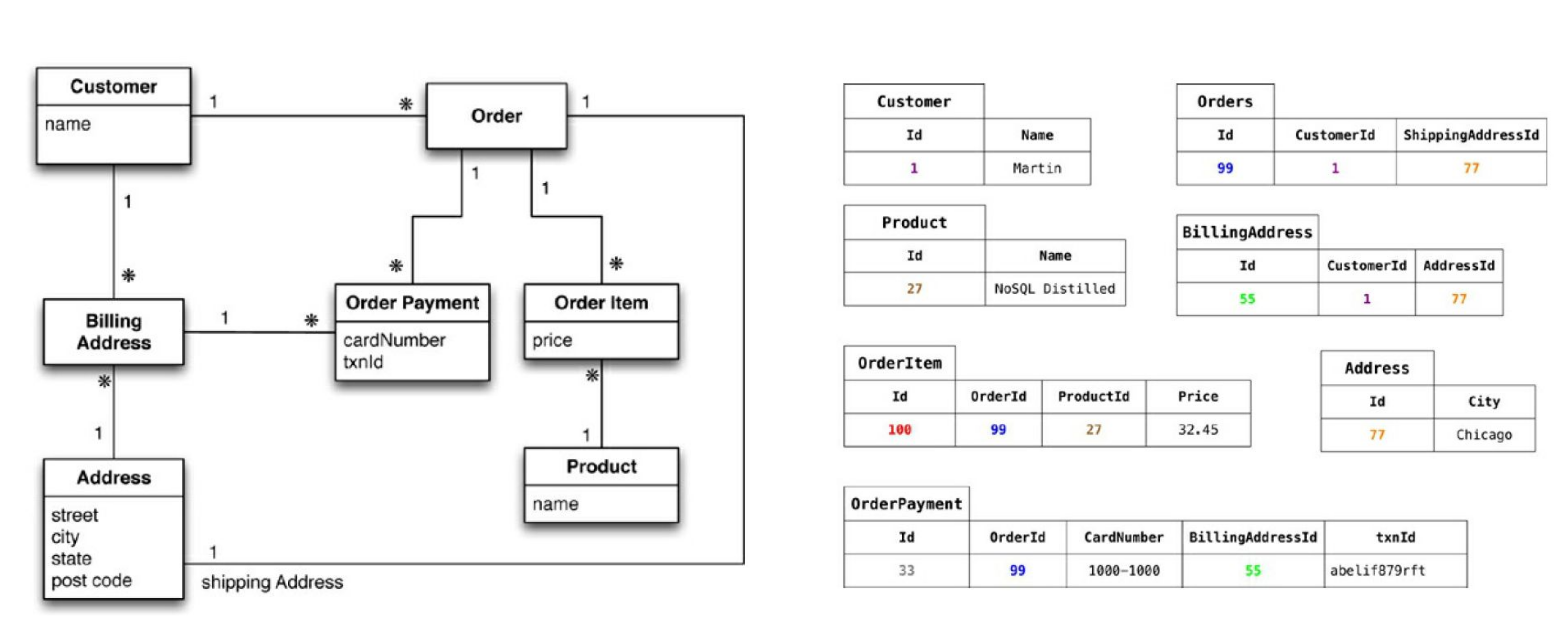
\includegraphics[width=1\textwidth]{dato_relacional.png}
			\caption{Modelo de datos relacional}
		\end{figure}
		
		
		\subsubsection{Aggregates}
		Es una forma para organizar y modelar los datos en sistemas NoSQL, como en algunas bases de datos orientadas a documentos. Un agregado es una unidad de datos autocontenida coherente que representa una entidad o idea en el dominio del problema. Se emplea para unir una variedad de objetos relacionados y sus relaciones en una sola unidad lógica.
		
		Permite romper la estructura limitada de las bases de datos relacionales y manipular los datos en unidades más complejas. Para organizar los datos de manera más adaptable y representar entidades relacionadas como una sola, se pueden anidar tuplas y listas de valores o tuplas.
		
		\begin{figure}[h]
			\centering
			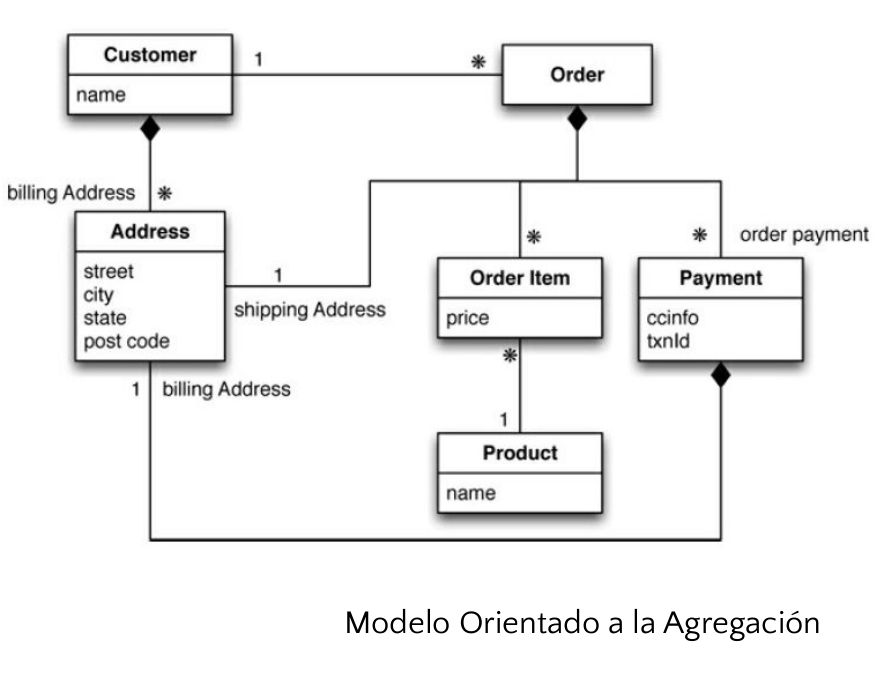
\includegraphics[width=0.5\textwidth]{aggregates.png}
			\caption{Modelo orientado a la agregación}
		\end{figure}
		
		\paragraph{Data models}
		\begin{itemize}
			\item {\textbf{Key-Value \& Document}}: Los aggregates se identifican (indexan) utilizando una clave o una identificación. En el modelo de Key-Value, el aggregate es opaco para la base de datos; por lo tanto, la base de datos simplemente trata el agregado como un gran "blob" sin estructura interna. Por otro lado, la base de datos impone condiciones y estructuras específicas para los aggregates en el modelo Documento, lo que permite un mayor acceso a través de consultas e índices relacionados con campos específicos.
			
			\item {\textbf{Key-Column-Family}}: Es una variante que organiza los aggregates utilizando una estructura de dos niveles. La primera clave identifica la fila o el conjunto de interés, y también se puede elegir la columna dentro del conjunto. Una familia de columnas incluye cada columna, y se supone que los datos de una familia de columnas se acceden normalmente en forma conjunta. Este modelo, que se basa en BigTable de Google, permite un almacenamiento optimizado para usos particulares.
		\end{itemize}
		\subsection{Modelos de Distribución}
		\subsubsection{Sharding}
		Es un método que permite a los usuarios acceder a diferentes partes de los datos en servidores individuales para reducir la carga y mejorar el rendimiento al distribuir diferentes partes de los datos en diferentes servidores. En resumen, la idea es colocar diferentes partes de los datos en diferentes servers.
		
		El caso ideal sería que cada usuario se comunique con un servidor específico para obtener una respuesta rápida y distribuir la carga de manera equitativa. Sin embargo, crear este caso ideal es difícil y requiere tener en cuenta una variedad de factores. Estos incluyen el criterio de distribución de datos entre nodos (como los apellidos A.D., E.F., R.Z.), el uso de zonas geográficas para reducir la latencia y el diseño de aggregates para agrupar datos relacionados.
		
		Los aggregates mejoran el rendimiento al acceder a datos juntos en el mismo servidor, pero también pueden reducir la robustez porque una falla de nodo puede causar la indisponibilidad parcial de datos.
		
		
		\subsubsection{Master-Slave Replication}
		Es una técnica utilizada en sistemas distribuidos para mejorar el rendimiento y la resistencia a fallos.
		
		Es un enfoque en el que un nodo se designa como el master o primario y recibe todas las operaciones de actualización. Los demás nodos son esclavos o secundarios, y la información se replica en ellos a partir de las actualizaciones realizadas en el master.
		
		Esto permite escalar en escenarios de alto tráfico de lecturas porque se distribuyen entre los esclavos, lo que alivia la carga del master debido a la reducción de lecturas. Además, mejora la resistencia a fallos porque otros nodos pueden seguir leyendo si un nodo falla. Sin embargo, como el master es un solo punto de falla, se debe tener un plan para restaurarlo en caso de falla.
		
		\subsubsection{Peer-to-Peer Replication}
		Es una táctica que aborda el problema del único punto de falla en la Master-Slave Replication. Este método no tiene un nodo principal y todas las réplicas son iguales. Cada nodo puede usar operaciones de lectura y escritura. Aunque esto mejora la resistencia a fallos, todavía hay inconsistencias de lectura transitorias.
		
		Sin un nodo central, pueden surgir conflictos de escritura cuando dos o más usuarios modifican el mismo registro al mismo tiempo en nodos diferentes. 
		
		Para manejar esto, hay dos alternativas:
		\begin{enumerate}
			\item {\textbf{Coordinar los nodos antes de realizar una escritura}}
			
			\item {\textbf{Soportar eventual inconsistencia}}
		\end{enumerate}
		
		
		
		\subsubsection{Sharding + Replication}
		Los datos se dividen en shards distribuidos en diferentes nodos para mejorar el rendimiento y la escalabilidad. Cada shard puede tener múltiples réplicas (maestros o esclavos) que se sincronizan para garantizar la alta disponibilidad y la tolerancia a fallos.
		
		\subsection{Consistencia}
		\subsubsection{Update Consistency}
		En un sistema de base de datos distribuido con replicación, como el caso de peer-to-peer replication, cada nodo puede recibir actualizaciones en un orden diferente, lo que podría conducir a diferentes valores finales para el mismo dato en diferentes nodos. Esta situación puede aumentar las posibilidades de conflicto write-write y llevar a inconsistencias en los datos.
		
		Para abordar la consistencia en actualizaciones, existen enfoques tanto pesimistas como optimistas. Los enfoques pesimistas intentan prevenir conflictos write-write mediante el uso de bloqueos de escritura (write-lock) para garantizar que solo un usuario pueda acceder al recurso a la vez. Sin embargo, esto puede afectar la escalabilidad y el rendimiento del sistema.
		
		Los enfoques optimistas, por otro lado, permiten que los conflictos ocurran pero los detectan y corrigen posteriormente. 
		Algunas tácticas optimistas comunes incluyen:
		\begin{enumerate}
			\item {\textbf{Conditional update}}: Cada usuario chequea el valor justo antes de actualizar, para ver si cambio
			luego de su última lectura.
			
			\item {\textbf{Almacenamiento de ambos updates}}: Almacenar ambos updates, indicar si se produce un conflicto, solicitar
			una solución al usuario (o hacerlo automáticamente si se puede).
		\end{enumerate}
		


		\subsubsection{Read Consistency}
		La consistencia en lecturas (read consistency) también puede ser un desafío debido a la posibilidad de conflictos read-write.
		
		Un conflicto read-write ocurre cuando un usuario (por ejemplo, B) realiza una lectura en medio de dos escrituras realizadas por otro usuario (por ejemplo, A). Esto puede resultar en una inconsistencia lógica en los datos, donde diferentes elementos de datos que tienen sentido en conjunto pueden leerse de manera descoordinada.
		
		Las transacciones en las bases de datos relacionales aseguran que un usuario lea los dos cambios realizados por A juntos o ninguno, lo que garantiza la consistencia lógica. Sin embargo, las cosas pueden ser diferentes en las bases de datos NoSQL, donde se utilizan actualizaciones atómicas a nivel de aggregates.
		
		Por ejemplo, en NoSQL, varios elementos de datos, incluidos precios de envío, ordenes y ítems, podrían formar parte del mismo aggregate. Si estos datos se almacenan en diferentes aggregates, puede haber una ventana de tiempo, también conocida como ventana de inconsistencia (inconsistency window), en la que se leerían valores inconsistentes.
		
		La replicación en sistemas distribuidos aumenta la ventana de inconsistencia, lo que afecta la consistencia lógica. Sin embargo, en muchos sistemas NoSQL se utiliza la consistencia eventual, lo que significa que tanto el usuario B como el usuario C leerán el valor correcto con el tiempo si no hay más actualizaciones. Esto se logra al permitir que las réplicas se establezcan con el tiempo.
		
		
		\subsubsection{Teorema CAP}
		El teorema CAP \footnote{también conocido como el Teorema de Brewer}, establece que en un sistema distribuido, es imposible garantizar simultáneamente las tres propiedades siguientes: Consistencia, Disponibilidad y Tolerancia al particionado. De acuerdo con el teorema, un sistema distribuido solo puede elegir dos de estas propiedades, pero no puede cumplir las tres al mismo tiempo.
		\begin{figure}[h]
			\centering
			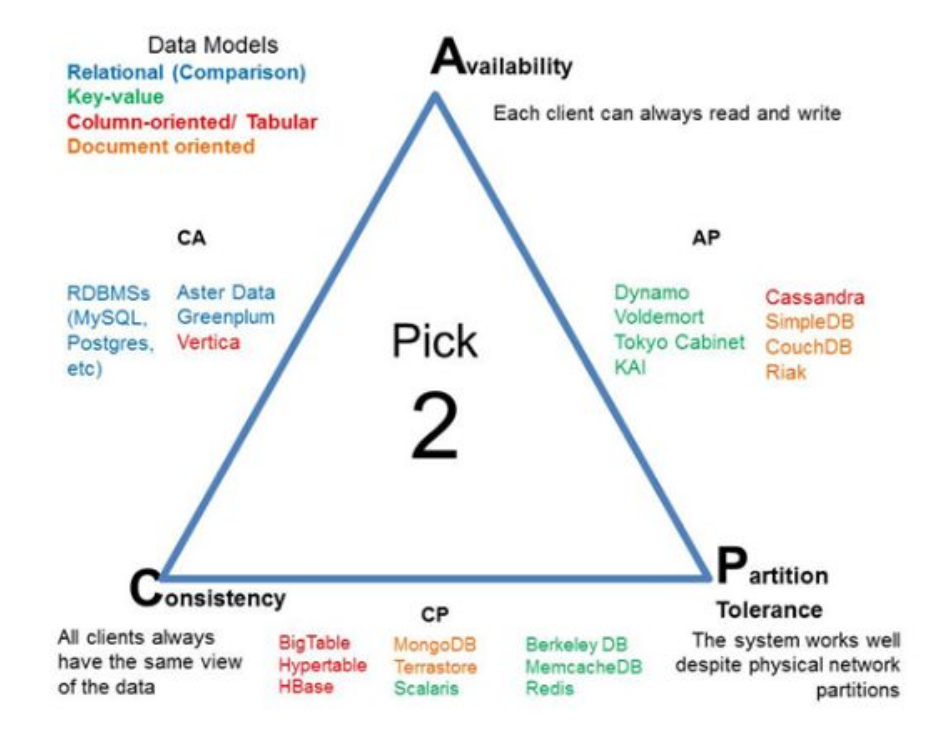
\includegraphics[width=0.5\textwidth]{teorema_cap.png}
			\caption{Teorema CAP}
		\end{figure}
		
		\pagebreak
		\begin{enumerate}
			\item {\textbf{Consistencia}}: Todos los nodos deben garantizar la misma información al	mismo tiempo.
			
			\item {\textbf{Disponibilidad}}: Cuando se hace	R/W en un nodo activo, este responde en tiempo acotado y sin errores.
			
			\item {\textbf{Tolerancia al particionado}}: ante una caída, el sistema sigue funcionando a pesar de que existan problemas de comunicación entre los nodos.
		\end{enumerate}
		
		
		
		
		\section{Patterns of Enterprise Application Architecture}
		Los sistemas de software conocidos como aplicaciones empresariales están diseñados para satisfacer las necesidades complejas y exigentes de las organizaciones empresariales. Debido a la gran cantidad de datos persistentes que deben gestionar y el acceso concurrente a los mismos, estas aplicaciones enfrentan numerosos desafíos. Además, deben proporcionar una variedad de vistas e interfaces de usuario para que los datos se presenten de manera adecuada a los diferentes usuarios y roles.
		
		Una característica clave de estas aplicaciones es la integración con otras aplicaciones comerciales, ya que suelen interactuar con varios sistemas y servicios para compartir datos y procesarlos. La lógica de negocios en las aplicaciones empresariales suele ser compleja y con frecuencia incluye varias reglas y flujos de trabajo.
		
		Se utilizan una variedad de patrones de diseño arquitectónico y de programación para organizar y estructurar el código de las aplicaciones empresariales. 
		
		\subsection{Organización lógica del Negocio}
		\subsubsection{Transaction Script}
		Es un patrón de diseño utilizado para gestionar la lógica de negocio de manera procedural o mediante funciones estáticas. En este patrón, cada acción o transacción se implementa como un procedimiento (script) independiente que procesa la entrada del usuario, accede a la base de datos, ejecuta la lógica del dominio y formatea el resultado para su presentación en la interfaz de usuario.
		\subsubsection{Domain Model}
		Es un enfoque de diseño orientado an objetos que se utiliza para representar y administrar la lógica comercial mediante objetos que reflejan las ideas del dominio del problema. Este patrón representa una clase para cada concepto o entidad del dominio, y cada instancia de la clase representa una ocurrencia específica del concepto.
		
		Además, el Domain Model facilita la representación fiel del dominio del problema, lo que mejora la comprensión y mantenimiento del código. 
		
		Sin embargo, el Domain Model tiene algunos inconvenientes. El mapeo complejo de objetos a la base de datos es uno de ellos. Puede requerir un esfuerzo adicional para definir las tablas, relaciones y consultas adecuadas para representar los objetos del modelo de dominio en una base de datos relacional.
		\subsubsection{Table Module}
		
		Es un patrón de diseño utilizado para organizar la lógica de negocio según la estructura de las tablas de la base de datos. En este patrón, se crea un módulo o clase para cada entidad de datos (o tabla) en la base de datos. Cada módulo contiene la lógica relacionada con esa entidad y proporciona métodos para interactuar con la base de datos a través de RecordSets.
		
		Dado que cada módulo representa una entidad de datos y agrupa todas las operaciones relacionadas con ella, Table Module facilita la organización de la lógica de dominio en la aplicación. Esto contribuye al mantenimiento de un código limpio y bien organizado.
		
		Además, una variedad de plataformas y lenguajes de programación ofrecen herramientas poderosas para trabajar con RecordSets, lo que facilita el manejo de los datos de la base de datos en la aplicación.
		
		No obstante, una de las desventajas de Table Module es que no aprovecha plenamente las ventajas de la programación orientada an objetos (OOP). Table Module no utiliza la herencia, el polimorfismo o la composición de objetos para representar conceptos de dominio, a diferencia de otros patrones de diseño orientados an objetos, como Domain Model. Por el contrario, su atención se centra en cómo están organizadas las tablas de la base de datos.
		
		La capacidad de los Table Module para generar duplicación de código es otra desventaja, ya que cada módulo contiene lógica específica para una entidad de datos específica. A medida que crece la aplicación, esto puede dificultar el mantenimiento y la escalabilidad del código.
		
		\subsubsection{Service Layer}
		Es un patrón de diseño que se utiliza para definir la frontera o interfaz de programación de aplicaciones (API) de la aplicación.
		
		El Service Layer se encarga de coordinar las respuestas a las solicitudes de los clientes, controlar los recursos transaccionales (si es necesario) y gestionar cualquier lógica de negocio que deba ocurrir antes o después de interactuar con el dominio.
		
		\subsection{Persistencia}
		\subsubsection{Arquitecturales}
		La persistencia en arquitectura se refiere al acceso y almacenamiento de datos en una aplicación. Para gestionar la persistencia, existen diferentes patrones arquitecturales que facilitan el acceso a recursos externos o bases de datos y la comunicación entre objetos independientes.
		\begin{enumerate}
			\item {\textbf{Gateway (Base Pattern)}}: Es un objeto que encapsula el acceso a un sistema externo o recurso. Actúa como una interfaz para acceder a la funcionalidad proporcionada por el recurso.
			
			
			
			\item {\textbf{Mapper (Base Pattern)}}:  Es un objeto que establece la comunicación entre dos objetos independientes. Su objetivo es transferir datos entre estos objetos
			
			\item {\textbf{Table Data Gateway}}: Este objeto actúa como un gateway para una tabla de base de datos, manejando todas las filas de la tabla. Se utiliza comúnmente en patrones como Transaction Script o Table Module.

            \item {\textbf{Row Data Gateway}}: Este objeto actúa como un gateway para un solo registro (fila) en una fuente de datos, teniendo una instancia por cada fila. También se emplea en patrones Transaction Script.
			
			\item {\textbf{Data Mapper}}: Es un objeto que envuelve una fila en una tabla o vista de una base de datos y encapsula el acceso a la base de datos, añadiendo lógica de dominio a esos datos. 
			
			
			
			\item {\textbf{Active Record}}: ante una caída, el sistema sigue funcionando a pesar de que existan problemas de comunicación entre los nodos.
		\end{enumerate}
		
		
		\subsubsection{Estructurales}
		La persistencia estructural se refiere al mapeo de la jerarquía de clases de un modelo de dominio a una jerarquía de tablas en una base de datos relacional.
		\paragraph{Jerarquías de asociación (composición / agregación)}
		
			\begin{enumerate}
			\item {\textbf{Identity Field}}: Es una técnica que guarda un identificador único de la base de datos (ID) en un objeto en memoria para mantener la identidad entre el objeto en la aplicación y la fila correspondiente en la tabla de la base de datos.
			
			
			\item {\textbf{Foreign-Key Mapping}}: Mapea una asociación entre objetos como una referencia de clave foránea (foreign key) entre tablas en la base de datos.
			
			\item {\textbf{Association Table Mapping}}: Guarda una asociación entre objetos como una tabla separada que contiene claves foráneas que enlazan las tablas de los objetos relacionados.
			
		\end{enumerate}

		\paragraph{jerarquías de herencia}
		
			\begin{enumerate}
				\item {\textbf{Single Table Inheritance}}: Representa una jerarquía de clases de herencia como una única tabla en la base de datos que contiene columnas para todos los campos de las diferentes clases.				
				
				\item {\textbf{Class Table Inheritance}}: Representa la jerarquía de clases de herencia con una tabla separada para cada clase.				
				
				
				\item {\textbf{Concrete Table Inheritance}}: Representa la jerarquía de clases de herencia con una tabla para cada clase concreta en la jerarquía.
				
			\end{enumerate}
		
		\subsubsection{Comportamiento}
		La persistencia de comportamiento se refiere a las estrategias utilizadas para manejar la carga diferida de datos y coordinar las operaciones de escritura y cambios en objetos en una base de datos.
		
		Algunos patrones de persistencia de comportamiento comunes son los siguientes:
		
			\begin{enumerate}
			\item {\textbf{Lazy Load}}: Es un patrón que permite cargar los datos de un objeto de manera diferida, es decir, solo cuando son necesarios. En lugar de cargar todos los datos de un objeto de inmediato, el objeto carga los datos a medida que se accede a ellos
			
			\item {\textbf{Unit of Work}}: Sirve para agrupar todas las operaciones relacionadas con una transacción de negocio en una única unidad lógica. Mantiene una lista de objetos afectados por la transacción y coordina la escritura de los cambios y la resolución de problemas de concurrencia
			
			
			\item {\textbf{Identity Map}}: Asegura que cada objeto se cargue solo una vez en memoria manteniendo una tabla hash (mapa) que almacena todos los objetos cargados.
			
		\end{enumerate}






  \section{Preguntas que me hicieron en el final}
  Si te toca Christian, muy probablemente te va a pedir definiciones. Si te toca Guille, te va a hacer pensar, pero es un tipazo.
   \subsection{Preguntas de Christian}
    \subsubsection{¿Qué es una SLA?}
    
    \textbf{\hyperlink{page.2}{Respuesta}}

    \subsubsection{¿Cuál es la diferencia entre escalabilidad y elasticidad?}

    La diferencia es que la escalabilidad es la capacidad del sistema para adaptarse al aumento de usuarios, transacciones y niveles de actividad, entre otros factores. 
    Y la Elasticidad se refiere a la capacidad de un sistema para adaptarse y ajustar sus recursos de manera dinámica y automática en respuesta a cambios en la carga de trabajo o demanda.


    \subsubsection{¿Qué dice la regla de los 5 9's?}

    Link: \textbf{\hyperlink{page.6}{Respuesta}}


    \subsubsection{¿Qué es el bandwidth?}

    Link: \textbf{\hyperlink{page.9}{Respuesta}}

    
    \subsubsection{¿Cuáles son las tácticas para la disponibilidad?}
    
    Link: \textbf{\hyperlink{page.7}{Respuesta}}

    \subsubsection{¿Cómo se pueden relacionar la arquitectura \textbf{stateless} con un \textbf{Load Balancer}?}
    
    Link: \hyperlink{page.23}{Respuesta: Tercer párrafo de Load Balancer}

    \subsubsection{¿Qué es la visibilidad?}
    
    Link: \hyperlink{page.14}{Respuesta}
    
    \subsubsection{¿Por qué las bases de datos relacionales no son escalables?}
    
    \hyperlink{page.45}{Link: \textit{Respuesta}}

    \subsubsection{¿Qué es Code On Demand?}
    
    \hyperlink{page.26}{Link: \textit{Respuesta}}


    \subsubsection{¿Qué es el sharding?}
    
    \hyperlink{page.43}{Link: \textit{Respuesta}}


   \subsection{Preguntas de Guille}
   
   \subsubsection{Si tuvieras un sistema como WhatsApp ¿qué atributos de calidad pensás que prioriza?}
    Acá la podes chamuyar, yo dije que priorizaba los siguientes: 
    \begin{itemize}
        \item Disponibilidad
        \item Perfomance
        \item Seguridad
        \item Portabilidad
    \end{itemize}

  \subsubsection{Si tuvieras otro sistema como un Home Banking ¿prioriza los mismo atributos que Whatsapp? ¿Cuáles cambia?}
    Acá haces lo mismo, la podes chamuyar, yo dije que no, no prioriza las mismas, dije que priorizaba los siguientes: 
    \begin{itemize}
        \item Seguridad
        \item disponibilidad
    \end{itemize}

    Porque realmente no importa si el homebanking es perfomante o no, como tambien con la portabilidad. 


  \subsubsection{¿Técnicas de disponibilidad?}
    Link: \textbf{\hyperlink{page.7}{Respuesta}}

  \subsubsection{¿Cómo es la arquitectura de Client-Stateless-Server?}
    Link: \textbf{\hyperlink{page.24}{Respuesta}}

  \subsubsection{Que un sistema sea stateless ¿beneficia a la escalabilidad? ¿O la perjudica? }
    Link: \textbf{\hyperlink{page.12}{Respuesta: En la parte de Tácticas}}

  \subsubsection{¿Qué es la HyperMedia en Rest?}
    Link: \textbf{\hyperlink{page.34}{Respuesta}}

    
  \subsubsection{¿Cuales son los riesgos de usar Cloud Computing?}
  El consumidor y el proveedor, con acceso privilegiado, tienen la responsabilidad de proteger sus datos. La dependencia de SLAs y la falta de controlabilidad en comparación con soluciones on-premise son problemas. La transferencia de datos entre proveedores cloud puede ser difícil, y las implicaciones legales, como la ubicación de datos y las leyes locales, plantean problemas. Debido a las leyes de ciertas jurisdicciones, existe el peligro de revelación no autorizada.

  \subsubsection{¿Qué es el auto-scaling? ¿Qué atributos de calidad favorece?}
    Link: \textbf{\hyperlink{page.41}{Respuesta}}

  \subsubsection{¿Por qué implementaria colas de mensajes entre los componentes?}
  
  Permiten el desacoplamiento entre componentes, lo que facilita la operación independiente y mejora la flexibilidad. Además, al procesar mensajes concurrentemente, administrar cargas variables y mejorar la capacidad de respuesta, promueven la escalabilidad horizontal. Al encolar y procesar mensajes lentamente, también son útiles para gestionar picos de carga, evitando la pérdida de datos o la degradación del rendimiento.

  \subsubsection{Si un worker agarra y procesa un pedido, y el worker falla en el medio ¿qué patrones podriamos implementar para arreglarlo?}
  Link: \textbf{\hyperlink{page.43}{Respuesta: Retry o Circuit Breaker}}

  \subsubsection{¿Qué es el sharding en NoSQL? ¿Puede haber replication sin sharding?}
  Link: \textbf{\hyperlink{page.48}{Respuesta: De sharding}} 

  Con respecto a la segunda pregunta: 

  Sí,  es posible sin sharding. La replicación crea copias de datos idénticas en varios nodos para garantizar la disponibilidad y la tolerancia a fallos. La replicación se enfoca en la redundancia y la disponibilidad, mientras que el sharding se enfoca en la distribución horizontal de los datos.



  \subsubsection{¿Cuáles son las formas de organizar la lógica de negocio?}
  Link: \textbf{\hyperlink{page.51}{Respuesta}} 

\end{document}